\documentclass[a4paper,12pt]{scrartcl}
\usepackage{pscyr}
\usepackage[14pt]{extsizes}
\usepackage{cmap}
\normalfont\normalsize
\usepackage[T2A]{fontenc}
\usepackage[utf8]{inputenc}
\usepackage[english,russian,ukrainian]{babel}
\usepackage{amssymb,amsfonts,amsmath,amsthm,mathtext,cite,enumerate,float}
\usepackage{indentfirst}
\usepackage{misccorr}
\usepackage{ccaption}
\usepackage{graphicx}
\usepackage{enumitem}
\usepackage{chngcntr}
\usepackage{makeidx}
\usepackage{framed}
\usepackage{lastpage}
\usepackage{longtable}
\usepackage{totcount}
\usepackage{etoolbox}
\usepackage{tabularx}
\usepackage{dsfont}
\usepackage{sectsty}
\usepackage{multirow}
\usepackage{gensymb}
\sectionfont{\fontsize{14}{14}\normalfont\bfseries}
\subsectionfont{\fontsize{14}{14}\normalfont\bfseries}
\subsubsectionfont{\fontsize{14}{14}\normalfont\bfseries}
\frenchspacing
\linespread{1.3}
\usepackage{geometry}
\geometry{left=3cm}
\geometry{right=1cm}
\geometry{top=2cm}
\geometry{bottom=2cm}
\geometry{footskip=\dimexpr\headsep+\ht\strutbox\relax}
\usepackage{titletoc}
\titlecontents{chapter}[0em]{\vskip12pt\bfseries\normalfont}
{\thecontentslabel\enspace}
{\hspace{1.05em}}
{\hfill\contentspage}[\vskip 3pt]
\titlecontents{section}[0em]{\normalfont}
{\thecontentslabel\enspace}
{}
{\titlerule*[1pc]{.}\quad\contentspage}[\vskip 4pt]
\titlecontents{subsection}[1em]{\normalfont}
{\thecontentslabel\enspace}
{}
{\titlerule*[1pc]{.}\quad\contentspage}[\vskip 3pt]
\dottedcontents{chapter}[1.6em]{}{1.6em}{1pc}
\setlist{nolistsep}
\setlength\parindent{5ex}
\graphicspath{{Mal/}}
\makeatletter
\renewcommand{\@biblabel}[1]{#1.}
\renewcommand*\verbatim@font{%
\normalfont\ttfamily
\hyphenchar\font\m@ne
\let\do\do@noligs\verbatim@nolig@list} 
\makeatother
\makeatletter
\newcommand{\verbatimfont}[1]{\def\verbatim@font{#1}}
\makeatother
\newtheoremstyle{algor}{3pt}{3pt}{}{5ex}{\bfseries}{.}{0.5em}{}
\theoremstyle{algor}
\newtheorem{algor}{Листинг}[section]
\counterwithin{table}{section}
\counterwithin{figure}{section}
\counterwithin{equation}{section}
\captiondelim{ - } % після точки стоїть пробіл!
%\captionnamefont{\large}
%\captiontitlefont{\large}
\makeindex
\makeatletter
\renewcommand{\@oddfoot}{\hfil \small \arabic{page}\hfil}
\renewcommand{\@evenfoot}{\hfil \small \arabic{page}\hfil}
\makeatother
\changecaptionwidth
\captionwidth{0.9\textwidth}
\captionstyle{\centering}
\usepackage{fancyhdr}
\pagestyle{fancy}
\fancyhf{}
\fancyhf[rh]{\thepage}% нумерація сторінок праворуч зверху
\renewcommand\headrulewidth{0pt}
\makeatletter % вирівнювання нижнього індексу
\newcommand{\subalign}[1]{%
  \vcenter{%
    \Let@ \restore@math@cr \default@tag
    \baselineskip\fontdimen10 \scriptfont\tw@
    \advance\baselineskip\fontdimen12 \scriptfont\tw@
    \lineskip\thr@@\fontdimen8 \scriptfont\thr@@
    \lineskiplimit\lineskip
    \ialign{\hfil$\m@th\scriptstyle##$&$\m@th\scriptstyle{}##$\crcr
      #1\crcr
    }%
  }
}
\makeatother
\newcounter{totfigures}
\newcounter{tottables}
\newcounter{totreferences}
\newcounter{totalgor}
\pretocmd{\section}{\addtocounter{totfigures}{\value{figure}}}{}{}
\pretocmd{\section}{\addtocounter{tottables}{\value{table}}}{}{}
\pretocmd{\section}{\addtocounter{totalgor}{\value{algor}}}{}{}
\pretocmd{\bibitem}{\addtocounter{totreferences}{1}}{}{}
\makeatletter
\AtEndDocument{%
\immediate\write\@mainaux{%
  \string\gdef\string\totfig{\number\value{totfigures}}%
  \string\gdef\string\tottab{\number\value{tottables}}% 
  \string\gdef\string\totalg{\number\value{totalgor}}% 
  \string\gdef\string\totref{\number\value{totreferences}}%
}%
}

\renewcommand\section{\@startsection {section}{1}{\z@}%
                                   {-3.5ex \@plus -1ex \@minus -.2ex}%
                                   {2.3ex \@plus.2ex}%
                                   {\centering\normalfont\bfseries}}


\usepackage{secdot}
\RequirePackage{caption}
\DeclareCaptionLabelSeparator{defffis}{ -- } % Разделитель
\captionsetup[table]{justification=raggedright, labelsep=defffis, format=plain, singlelinecheck=false} % Подпись таблицы слева
\captionsetup[figure]{justification=centering, labelsep=defffis, format=plain} % Подпись рисунка по центру

% Костыль для содержания
\usepackage[compact,explicit]{titlesec}
%\usepackage{etoolbox}

\makeatletter
\patchcmd{\ttlh@hang}{\parindent\z@}{\parindent\z@\leavevmode}{}{}
\patchcmd{\ttlh@hang}{\noindent}{}{}{}
\makeatother


\titleformat{\section}{\bfseries}{}{12.5mm}{\centering{\thesection\quad\bfseries{#1}}\vspace{1.5em}}
\titleformat{\subsubsection}[block]{\vspace{1em}\bfseries\normalsize}{}{12.5mm}{\thesubsubsection\;\bfseries#1\vspace{1em}}
\titleformat{\subsection}[block]{\bfseries\vspace{1pt}}{}{12.5mm}{\thesubsection\bfseries\;#1\vspace{1em}}

\titlespacing{\subsection}{0\parindent}{0.5em}{0em}
\titlespacing{\subsubsection}{0\parindent}{-0.5em}{0em}

\makeatother

% Секции без номеров (введение, заключение...), вместо section*{}
\newcommand{\anonsection}[1]{
    %\phantomsection % Корректный переход по ссылкам в содержании
    \paragraph{\centerline{{#1}}\vspace{1.5em}}
    %\addcontentsline{toc}{section}{\uppercase{#1}}
}

\makeatletter
\def\hlinewd#1{%
  \noalign{\ifnum0=`}\fi\hrule \@height #1 \futurelet
   \reserved@a\@xhline}
\makeatother

\usepackage{tocloft}
\renewcommand{\cfttoctitlefont}{\bfseries\hspace{0.38\textwidth}} % СОДЕРЖАНИЕ
\renewcommand{\cftsecfont}{\hspace{0pt}}            % Имена секций в содержании не жирным шрифтом
\renewcommand\cftsecleader{\cftdotfill{\cftdotsep}} % Точки для секций в содержании
\renewcommand\cftsecpagefont{\mdseries}             % Номера страниц не жирные
\setcounter{tocdepth}{3}                            % Глубина оглавления, до subsubsection

\usepackage{fancyhdr}
\pagestyle{fancy}
\fancyhf{}
\fancyhead[R]{\textrm{\thepage}}
\fancyheadoffset{0mm}
\fancyfootoffset{0mm}
\setlength{\headheight}{17pt}
\renewcommand{\headrulewidth}{0pt}
\renewcommand{\footrulewidth}{0pt}
\fancypagestyle{plain}{ 
    \fancyhf{}
    \rhead{\thepage}
}

% Списки
\usepackage{enumitem}

\begin{document}
\def\figurename{Рисунок}
\def\tablename{Таблиця}
\verbatimfont{\ttfamily}
\let\normalint\int % PS
\def\int{\displaystyle\normalint} %PS
\let\normaliint\iint % PS
\def\iint{\displaystyle\normaliint} %PS
\let\normaliiint\iiint % PS
\def\iiint{\displaystyle\normaliiint} %PS
\let\normalsum\sum % PS
\def\sum{\displaystyle\normalsum} %PS
\renewcommand{\contentsname}{ЗМІСТ}

\pretolerance10000

\setlist[enumerate,itemize]{listparindent=18mm, leftmargin=18mm} % Отступы в списках
%\anonsection{Реферат}
\label{sec:Refer}


\hspace*{26pt} У роботі проводиться розрахунок площі криволінійного паркану змінної висоти. Висота задається як функція декартових координат точки паркана.

Пошук алгоритмів розв’язання задачі виконаний на сайті \cite{GoogleWebPage}. Для обчислення площі використовуються криволінійні інтеграли 1-го роду \cite{Senchuk2006}. Чисельні приклади розв’язані у MATLAB \cite{Anufriev2005}. Використовувалася також сторінка \cite{IglinWebPage}.

\vspace{0.25cm}

Іл.\,\totfig. Табл.\,\tottab. Лист.\,\totalg. Бібліогр.:\,\totref\,назв.



%\newpage
%\tableofcontents
%\newpage
%%\anonsection{Перелік позначень та скорочень}
\anonsection{ПЕРЕЛІК ПОЗНАЧЕНЬ ТА СКОРОЧЕНЬ}
\addcontentsline{toc}{section}{Перелік позначень та скорочень}


\hspace*{26pt}


%\newpage
%%\anonsection{Вступ}
\anonsection{ВСТУП}
\addcontentsline{toc}{section}{Вступ}



Термін самонавчання (self-supervised learning, SSL) використовувався у різних контекстах та сферах, таких як навчання уявлень (representation learning), нейронні мережі, робототехніка, обробка природних мов (natural language processing, NLP) та навчання з посиленням (reinforcement learning). У всіх випадках основна ідея полягає в тому, щоб автоматично генерувати якийсь наглядовий сигнал для вирішення якогось завдання (як правило, вивчати подання даних або автоматично розмічати набір даних).

В типовій задачі SSL є величезна нерозмічена вибірка, необхідно сформувати для кожного об'єкта псевдо-мітку (pseudo label) і вирішити отриману SSL-завдання, але нас цікавить не стільки якість рішення придуманого нами завдання (її називають pretext task), скільки представлення (representation) об'єктів, яке буде вивчено в процесі її рішення. Це представлення можна в подальшому використовувати вже при вирішенні будь-якої задачі з мітками (SSL), яку називають наступною задачею (downstream task). Одна з головних причин самонавчання $-$ невеликий обсяг розмічених даних. На відміну від навчання з частково розміченими даними в самонавчанні використовуються абсолютно довільні нерозмічену дані, що не мають відношення до розв'язуваної задачі.

Сучасна обробка тексту (NLP) приблизно на 80\% складається з самонавчання. Наприклад, за допомогою самонавчання можна знайти майже всі представлення слів (а також текстів). Наприклад, в класичному алгоритмі word2vec беруть нерозмічений корпус текстів, потім самі придумують завдання з мітками (по сусіднім словами передбачити центральне слово або, навпаки, по центральному сусідні з ним), навчають на цьому завданні просту нейронну мережу, в результаті виходять векторні уявлення слів, які вже використовуються в інших, ніяк не пов'язаних з попередньою, задачах. Часто такий підхід називають також трансферним навчанням (transfer learning). Вцілому, трансферне навчання більш широке поняття - коли модель, навчену для вирішення однієї задачі, використовують при вирішенні іншої. У самонавчанні важливо, щоб розмітка в попередньої задачі (псевдо-мітки) виходила автоматично. Наприклад, представлення, отримані методом Cove, в якому використовується кодер для завдання машинного перекладу, будуть трансферними, але не отриманими за допомогою самонавчання.

Останнім часом, набирає популярність підрозділ самонавчання $-$ порівняльне навчання (constrastive learning).

Метою даної дипломної роботи є дослідження роботи алгоритмів порівняльного навчання Deep InfoMax та Momentum Contrast.


%\newpage
%%\section{Огляд літературних джерел}
\section{ОГЛЯД ЛІТЕРАТУРНИХ ДЖЕРЕЛ}
\label{sec:Theory}

Самонавчання дає нам змогу безкоштовно використовувати різноманітні позначки, що постачаються з даними. Мотивація досить проста: нерозмічених даних дуже багато і їхня кількість постійно зростає, в той час як процес розмаркування даних доволі затратний, як з точки зору часу так і людських ресурсів. Щоб використовувати набагато більшу кількість немаркованих даних, одним із способів є правильне встановлення цілей навчання, щоб отримати контроль від самих даних.

До основних понять самоначання можна віднести:

\begin{enumerate}
	\item попередня задача (pretext task) $-$ задача з штучно створеними мітками (псевдо-мітками), на якій навчається модель, щоб вивчити хороші представлення (representations) об'єктів;
	\item псевдо-мітки (pseudo labels) $-$ мітки, що ми можемо формувати автоматично, без ручної розмітки, але навчання яким сприяє формуванню хороших представлень;
	\item подальша задача (downstream task) $-$ задача на якій перевіряють якість отриманих представлень. 
\end{enumerate}
		
Майже у всіх експериментах в статтях по самонавчання на отриманих ознакових представленнях в наступних завданнях навчають прості моделі: логістичну регресію або метод найближчого сусіда. Таким чином, самонавчання $-$ це напрямок в глибокому навчанні, який прагне зробити глибоке навчання процедурою попередньої обробки даних, тобто мережі потрібні для формування ознак, вони навчаються на дешевій розмітці великих наборів спочатку нерозмічену даних, а сама задача вирішується простою моделлю.

\subsection{Порівняльне навчання}

В останні роки значно менше робіт з вибору попередніх завдань, оскільки основним напрямком в самообучении стало порівняльне навчання (Contrastive Learning). На вхід нейромережі подається пара об'єктів і вона визначає, схожі вони чи ні. Якщо об'єкт подається як аугментований патч з зображення, патчі однієї природи мають бути схожи, а різної $-$ несхожі. В якості оптимізуємої функції використовується взаємна інформація або пов'язані з нею функції, наприклад, її нижня оцінка InfoNCE :

\begin{equation}\label{eq:infonce}
-E_{x}\left[ \log{\frac{exp(f(x)^{T}f(x^{+}))}{exp(f(x)^{T}f(x^{+}))+\sum_{j=1}^{N-1}exp(f(x)^{T}f(x_{j}))}} \right],
\end{equation}

\noindent де $x$ $-$ обраний патч, званий якірним, \newline
\hspace*{15pt} $x^{+}$ $-$ схожий на нього, \newline
\hspace*{15pt} $x_{j}$ $-$ несхожий (їх $N-1$ штука), \newline
\hspace*{15pt} $f()$ $-$ кодер об'єкту. 

\vspace{1.5em}

Така функція помилки майже перетворюється в Triplet Loss, якщо використовувати тільки 1 негативний приклад.

Розглянемо певні алгоритми порівняльного навчання.

\subsection{Deep InfoMax}

Окреслимо загальні параметри навчання кодеру для максимізації взаємної інформації між його входом і виходом. Нехай $X$ і $Y$ є областю визначення і областю значень неперервної та (майже скрізь) диференційованої параметричної функції, $E_{\psi}: X \rightarrow Y$ з параметрами $\psi$ (наприклад, нейронна мережа). Ці параметри визначають сімейство кодерів $E_{\Psi} = {E_{\phi}}_{\psi \in \Psi}$ над $\Psi$ (множина нейронних мереж). Припустимо, що нам дано набір навчальних прикладів на вхідному просторі, $X$: $\mathbf{X} := {x^{(i)} \in X}^{N}_{i = 1}$, з емпіричним розподілом ймовірностей $\mathbb{P}$. Визначимо $\mathbb{U_{\psi,P}}$ як граничний розподіл, індукований проштовхуванням зразків від $\mathbb{P}$ через $\mathbb{E_{\psi}}$. Тобто, $\mathbb{U_{\psi, P}}$ $-$ розподіл за кодуваннями $y \in Y$, отриманий шляхом вибірки спостережень $x \sim X$, а потім вибірки $y \sim E_{\psi}(x)$ [4].

Приклад кодера даних зображень наведено на рис. \ref{fig:deepinfo1}, який буде використаний у наступних розділах, але цей підхід можна легко адаптувати для тимчасових даних. 

\newpage

\vspace{1em}

\begin{figure}[h]
  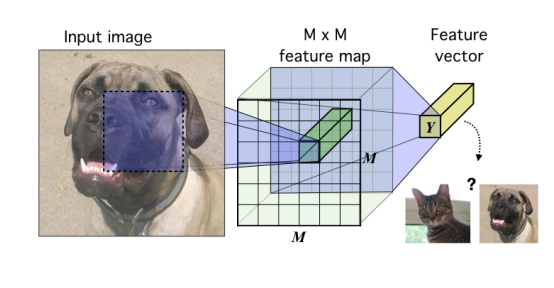
\includegraphics[width=\textwidth, height=5cm, natwidth=277, natheight=144]{Mal/deepinfo1.jpg}
  \caption{Базова модель кодера в контексті саних зображень.}
  \label{fig:deepinfo1}
\end{figure}

Подібно до принципу оптимізації infomax, можна стверджувати, що кодер повинен навчатися відповідно до таких критеріїв:

\begin{enumerate}
	\item максимізація взаємної інформації; 
	\item статистичні обмеження. 
\end{enumerate}


Максимізація взаємної інформації полягає в тому, що необхідно знайти набір параметрів $\psi$, таких, щоб взаємна інформація $L(X; E_{\psi} (X))$ була максимальною. Залежно від кінцевої цілі, ця максимізація може бути здійснена за повним входом $X$, або деякою структурованою або «локальною» підмножиною.

В той час як статистичні обмеження відповідають за те, що залежно від кінцевої мети для подання, граничні $\mathbb{U}_{\psi, \mathbb{P}}$ повинні відповідати апріорному розподілу ймовірності $\mathbb{V}$. Грубо кажучи, це може бути використано для заохочення вихідних даних кодера до бажаних характеристик (наприклад, незалежності).

Формулювання цих двох цілей називається Deep InfoMax (DIM) [4].

\subsubsection{Оцінка та максимізація взаємної інформації}

Основні рамки максимізації взаємної інформації представлені на рис. \ref{fig:deepinfo2}. 

\vspace{1em}

\begin{figure}[h]
  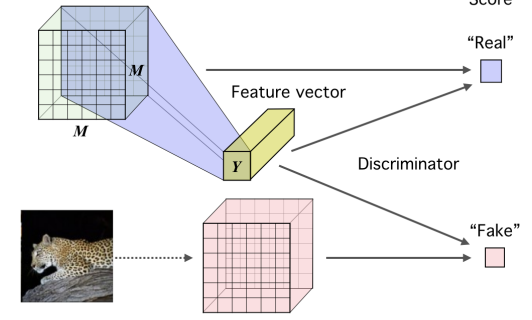
\includegraphics[width=\textwidth, height=5cm, natwidth=266, natheight=160]{Mal/deepinfo2.jpg}
  \caption{Deep InfoMax (DIM) з глобальною MI(X; Y) ціллю.}
  \label{fig:deepinfo2}
\end{figure}

Підхід слідує взаємній інформаційній нейронній оцінці (MINE), яка оцінює взаємну інформацію шляхом підготовки класифікатора для розрізнення зразків, що надходять із спільного розподілу $\mathbb{J}$ та відособленого розподілу $\mathbb{M}$ випадкових величин $X$ та $Y$. MINE використовує нижню межу для спільної інформації MI (від англійського mutual information) на основі представлення Донскер$-$Варадхана (DV) KL-дивергенції:

\begin{equation}\label{eq:dv}
L(X; Y) := D_{KL}(\mathbb{J}||\mathbb{M}) \ge \hat{L}_{\omega}^{DV}(X;Y):=\mathbb{E}_{\mathbb{F}}|T_{\omega}(x,y)| - \log{\mathbb{E}_{\mathbb{M}}[e^{T_{\omega}(x,y)}}],
\end{equation}

\noindent де $T_{\omega}: X \times Y \rightarrow \mathbb{R}$ функція дискримінатора, змодельована нейронною\newline 
\hspace*{15pt}мережею з параметрами $\omega$.

\vspace{1.5em}

На найвищому рівні оптимізується $\mathbb{E_{\psi}}$ одночасно оцінюючи та максимізуючи $L(X, E_{\psi}(X))$,

\begin{equation}\label{eq:e_psi_opt}
(\hat{\omega}, \hat{\psi})_{G} = \underset{\omega,\psi}{\arg\max}\hat{L}_{\omega}(X;E_{\psi}(X)),
\end{equation}

\vspace{1.5em}

\noindent де нижній індекс $G$ позначає «глобальний». 

Однак існують деякі важливі відмінності, які відрізняють цей підхід від MINE. По-перше, оскільки кодер і оцінювач взаємної інформації оптимізують одну і ту ж мету і вимагають подібних обчислень, ми ділимо шари між цими функціями, так що: 

\begin{equation}\label{eq:hz}
	E_{\psi} = f_{\psi} \circ C_{\psi} \, \text{та} \, T_{\psi, \omega} = D \circ g \circ (C_{\psi}, E_{\psi}), 
\end{equation}

\noindent де $g$ - функція, яка поєднує вихідні дані кодера з нижчим шаром.

\vspace{1.5em}

По-друге, враховуючи зацікавленність в максимальному збільшенні MI і не турбуючись його точним значенням, можна покластися на розбіжності, не пов’язані з KL, які можуть запропонувати вигідні компроміси. Наприклад, можна визначити оцінювач МІ Дженсена-Шеннона:

\begin{eqnarray}\label{eq:mi}
%\begin{aligned}
\hat{L}_{\omega, \psi}^{(infoNCE)}(X;E_{\psi}(X)) := \\ := \mathbb{E_{P}}\left[T_{\psi,\omega}(x, E_{\psi}(x)) - \mathbb{E_{\tilde{P}}}\left[\log{\sum_{x'}{e^{T_{\psi, \omega}(x',E_{\psi}(x))}}}\right]\right],
%\end{aligned}
\end{eqnarray}

\noindent де $x$ $-$ вхідний зразок, \newline
\hspace*{15pt} $x'$ $-$ вхід, відібраний з $\tilde{\mathbb{P}} = \mathbb{P}$, \newline
\hspace*{15pt} $sp(z) = \log{(1 + e^{z})}$ $-$ функція softplus. 

\vspace{1.5em}

Подібний оцінювач з'явився у контексті мінімізації сумарної кореляції, і це становить знайому двійкову перехресну ентропію. Це добре розуміється з точки зору оптимізації нейронних мереж, що на практиці такий підхід працює краще (наприклад, є стабільнішим), ніж ціль на основі DV. Інтуїтивно оцінювач, що базується на Йенсена-Шеннона, повинен поводитись подібно до оцінювача, що базується на DV в рівнянні. \ref{eq:mi}, оскільки обидва діють як класифікатори, цілі яких максимізують очікуване $log$-співвідношення з'єднання над добутком маржиналів.

Оцінка контрастності шуму (Noise-Contrastive Estimation) також може використовуватися з DIM шляхом максимізації:

\begin{equation}\label{eq:dim}
\hat{L}_{\omega,\psi}^{infoNCE}(X; E_{\psi}(X)) := \mathbb{E_{P}}\left[T_{\psi,\omega}(x, E_{\psi}) - \mathbb{E_{\tilde{P}}}\left[\log{\sum_{x'}{e^{T_{\psi, \omega}(x', E_{\psi}(x))}}}\right]\right].
\end{equation}

\vspace{1.5em}

Для DIM ключовою різницею між формулюваннями DV, JSD та infoNCE є те, чи з'являється очікування над $\mathbb{P / \tilde{P}}$ всередині $log$ або поза ним. Насправді ціль, що базується на JSD, відображає оригінальну формулювання NCE, яка формулює ненормалізовану оцінку щільності як двійкову класифікацію між розподілом даних та розподілом шуму. DIM встановлює розподіл шуму на добуток граничних значень на $X / Y$, а розподіл даних $-$ на справжнє з'єднання. Формулювання infoNCE слідує версії NCE на основі softmax, подібній до тих, що використовуються у спільноті моделювання мов і яка має міцні зв'язки з бінарною перехресною ентропією в контексті поріввняльного навчання. На практиці реалізації ці оцінювачи здаються досить схожими і можуть повторно використовувати більшість того самого коду. Дослідження JSD та infoNCE у експериментах дозволяє виявити, що використання infoNCE часто перевершує JSD у подальших завданнях, хоча цей ефект зменшується із більш складними даними. Однак для того, щоб infoNCE та DV вимагали великої кількості негативних зразків (зразки з $\mathbb{\tilde{P}}$), вони повинні бути конкурентоспроможними.

\subsubsection{Максимізація локальної спільної інформації}

Критерій в рівнянні \ref{eq:e_psi_opt}  можна використовувати для максимізації MI між входом і виходом, але в кінцевому рахунку це може бути небажаним залежно від завдання. Наприклад, тривіальний шум на рівні пікселів марний для класифікації зображень, тому подання може не отримати вигоди від кодування цієї інформації (наприклад, при навчанні з нульовим знімком, навчанні передачі тощо). Для того, щоб отримати представлення, більш придатне для класифікації, можна замість цього максимізувати середній MI між представленням високого рівня та локальними плямами зображення. Оскільки одному і тому ж представництву рекомендується мати високий MI з усіма патчами. це надає перевагу кодуванню аспектів даних, які спільно використовуються між патчами.

Припустимо, що вектор ознак має обмежену ємність (кількість одиниць та діапазон) і припустимо, що кодер не підтримує нескінченні вихідні конфігурації. Для максимізації MI між усім входом і поданням, кодер може вибрати який тип інформації на вході передається через кодер, наприклад, шум, характерний для локальних латок або пікселів. Однак, якщо кодер передає інформацію, характерну лише для деяких частин вводу, це не збільшує МІ з будь-якими іншими патчами, які не містять згаданого шуму. Це спонукає кодер віддавати перевагу інформації, яка передається у вхідних даних [4].

DIM-фреймворк представлено на рис. \ref{fig:deepinfo3}. 

\vspace{1em}

\begin{figure}[h]
  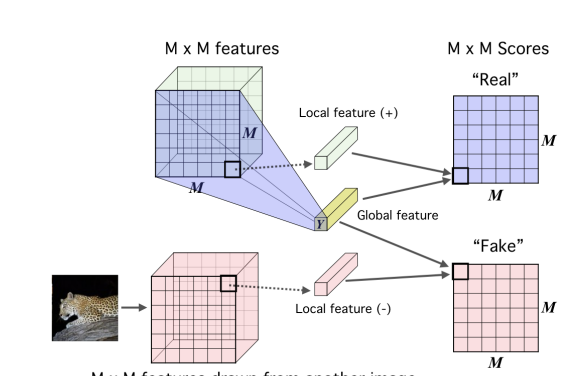
\includegraphics[width=\textwidth, height=5cm, natwidth=291, natheight=188]{Mal/deepinfo3.jpg}
  \caption{Максимізація взаємної інформації між локальними та глобальними характеристиками.}
  \label{fig:deepinfo3}
\end{figure}

Спочатку потрібно закодувати вхідні дані до карти об’єктів, $C_{\psi} = \left\{ C_{\psi}^{(i)} \right\}_{i=1}^{M \times M}$, що відображає корисну структуру в даних, індексовану в цьому випадку $i$. Далі, можна узагальнити цю локальну карту об’єктів у загальну характеристику: $E_{\psi} = f_{\psi} \circ C_{\psi}(x)$. Потім необхідно визначити оцінювач MI на глобальних та локальних парах, максимізуючи середню оцінку MI:

\begin{equation}\label{eq:max_mi}
(\hat{\omega}, \hat{\psi})_{L} = \underset{\omega,\psi}{\arg\max}\frac{1}{M^{2}}\sum_{i=1}^{M^{2}}\hat{L}_{\omega, \psi}(C_{\psi}^{(i)}(X); E_{\psi}(X)).
\end{equation}

\vspace{1.5em}

\subsubsection{Відповідність представлень апріорному розподілу}

Абсолютна величина інформації є лише однією бажаною властивістю уявлення. Залежно від програми хороші уявлення можуть бути компактними, незалежними, розплутаними або незалежно керованими. DIM накладає статистичні обмеження на вивчені уявлення, неявно навчаючи кодер так, щоб образ міри $\mathbb{U_{\psi, P}}$ збігався з попереднім $\mathbb{V}$. Це робиться шляхом навчання дискримінатора, $D_{\phi} : Y \rightarrow \mathbb{R}$, для оцінки розбіжності, $D(\mathbb{V} || \mathbb{U_{\psi, P}})$. Після чого тренуємо кодер для мінімізації оцінки:

\begin{eqnarray}\label{eq:div}
%\begin{aligned}
(\hat{\omega}, \hat{\psi})_{P} \underset{\psi}{\arg\min}\,\underset{\phi}{\arg\max}\hat{D}_{\phi}(\mathbb{V}||\mathbb{U_{\psi,P}}) = \mathbb{E_{V}}[\log{D_{\phi}(y)}] + \\ + \mathbb{E_{P}}[\log{(1-D_{\phi}(E_{\psi}(x)))}].
%\end{aligned}
\end{eqnarray}

\vspace{1.5em}

Цей підхід подібний до того, що робиться в змагальних автокодерах, але без генератора. Він також схожий на шум як цілі, але тренує кодер, щоб він неявно відповідав шуму, а не використовував апріорні вибірки шуму як цілі.

Всі три цілі: глобальна та локальна максимізація МІ та попереднє узгодження можуть бути використані разом. І, таким чином, можна отримати критерій Deep InfoMax (DIM):

\begin{eqnarray}\label{eq:deepinfomax}
%\begin{aligned}
\underset{\omega_{1},\omega_{2},\psi}{\arg\max}(\alpha \hat{L}_{\omega_{1},\psi}(X; E_{\psi}(X)) + \frac{\beta}{M^{2}}\sum_{i=1}^{M^{2}}{\hat{L}_{\omega_{2}, \psi}(X^{(i)}; E_{\psi}(X)))} + \\
+ \underset{\psi}{\arg\min}\,\underset{\phi}{\arg\max}\gamma\hat{D}_{\phi}(\mathbb{V}||\mathbb{U_{\psi,P}}),
%\end{aligned}
\end{eqnarray}

\noindent де $\omega_{1}$ та $\omega_{2}$ $-$ параметри дискримінатора відповідно до глобальних \newline
\hspace*{15pt}та локальних цілей, \newline
\hspace*{15pt}$\alpha$, $\beta$ та $\gamma$ $-$ гіперпараметри.

\vspace{1.5em}

\subsection{Momentum Contrast}

Порівняльне навчання та його останні розробки можна розглядати як навчання кодеру для завдання пошуку у словнику.

Розглянемо закодований запит $q$ та набір закодованих зразків $\{k_{0}, k_{1}, k_{2}, \dots\}$, які є ключами словника. Припустимо, що у словнику є один ключ (позначений як $k_{+}$), який відповідає $q$. Контрастивна втрата $-$ це функція, значення якої є низьким, коли $q$ подібне до його позитивного ключа $k_{+}$ та відрізняється від усіх інших ключів (вважається негативним ключем для $q$). Можна перевизначити функцію InfoNCE:

\begin{equation}\label{eq:infonce_simple}
L_{q} = -\log{\frac{exp(q \cdot k_{+}/\tau)}{\sum_{i=0}^{K}{exp(q \cdot k_{i}/\tau)}}},
\end{equation}

\vspace{1.5em}

\noindent де $\tau$ гіперпараметр. 

Сума складається з однієї позитивної та $K$ негативних екземплярів. Інтуїтивно, ця втрата є логаріфмічною втратою класифікатора на основі $(K + 1)$ softmax, який намагається класифікувати $q$ як $k_{+}$. Функції контрастивних збитків можуть також базуватися на інших формах, таких як маржові збитки та варіанти збитків NSE.

Контрастивна втрата служить неконтрольованою цільовою функцією для навчання мереж кодера, що представляють запити та ключі. Загалом, подання запиту має значення $q = f_{q} (x^{q})$, де $f_{q}$ - це мережа кодера, а $x^{q}$ - зразок запиту (так само, $k = f_{k} (x^{k})$). Їх екземпляри залежать від конкретного попередньогозавдання. Вхідними даними $x^{q}$ та $x^{k}$ можуть бути зображення, патчі або контекст, що складається з набору патчів. Мережі $f_{q}$ і $f_{k}$ можуть бути ідентичними, частково спільними або різними.

З вищенаведеної точки зору, порівняльне навчання $-$ це спосіб побудови дискретного словника на безперервних вхідних даних, таких як зображення. Словник є динамічним у тому сенсі, що ключі вибираються випадково, а кодер ключів розвивається під час навчання. Гіпотеза полягає в тому, що хорошим можливостям можна навчитися за допомогою великого словника, який охоплює багатий набір негативних зразків, тоді як кодер ключів словника зберігається якомога послідовнішим, незважаючи на його розвиток. Виходячи з цього можна описати алгорим Momentum Contrast.

В основі цього підходу лежить підтримка словника як черги зразків даних. Це дозволяє нам повторно використовувати закодовані ключі з безпосередніх попередніх міні-пакетів. Введення черги відокремлює розмір словника від розміру міні-партії. Розмір словника може бути набагато більшим, ніж типовий розмір міні-партії, і може бути гнучко та незалежно встановлений як гіперпараметр.

Зразки у словнику поступово замінюються. Поточна міні-партія потрапляє до словника, а найстаріша міні-партія в черзі вилучається. Словник завжди представляє вибіркову підмножину всіх даних, тоді як додаткові обчислення ведення цього словника є керованими. Більше того, видалення найстарішої міні-партії може бути корисним, оскільки її закодовані ключі є найбільш застарілими і, отже, найменш відповідають найновішим.

Використання черги може зробити словник великим, але це також робить важким оновлення кодера ключа шляхом зворотного розповсюдження (градієнт повинен поширюватися на всі зразки в черзі). Наївним рішенням є копіювання кодера ключа $f_{k}$ з кодера запиту $f_{q}$, ігноруючи цей градієнт. Але це рішення дає погані результати в експериментах. Припустимо, що такий збій спричинений швидко мінливим кодером, який зменшує узгодженість ключових подань. Пропонується оновити імпульс для вирішення цієї проблеми.

Формально, позначаючи параметри $f_{k}$ як $\theta_{k}$, а параметри $f_{q}$ як $\theta_{q}$, ми оновлюємо $\theta_{k}$ за допомогою:

\begin{equation}\label{eq:theta_opt}
\theta_{k} \leftarrow m\theta_{k} + (1 - m)\theta_{q}.
\end{equation}

\vspace{1.5em}

Тут $m \in [0, 1)$ $-$ коефіцієнт імпульсу. Тільки параметри $\theta_{q}$ оновлюються шляхом зворотного розповсюдження. Оновлення імпульсу в рівнянні \ref{eq:theta_opt} змушує $\theta_{k}$ еволюціонувати більш плавно, ніж $\theta_{q}$. Як результат, хоча ключі в черзі кодуються різними кодерами (в різних міні-партіях), різниця між цими кодерами може бути невеликою. В експериментах порівняно великий імпульс (наприклад, m = 0,999, за замовчуванням) працює набагато краще, ніж менший показник (наприклад, m = 0,9), що дозволяє припустити, що кодер ключів, який повільно розвивається, є стрижнем для використання черги.

MoCo $-$ загальний механізм використання контрастивних втрат. Ми порівнюємо це з двома існуючими загальними механізмами на рис \ref{fig:momentum1}. Вони мають різні властивості щодо розміру та послідовності словника.

\vspace{1em}

\begin{figure}[h]
  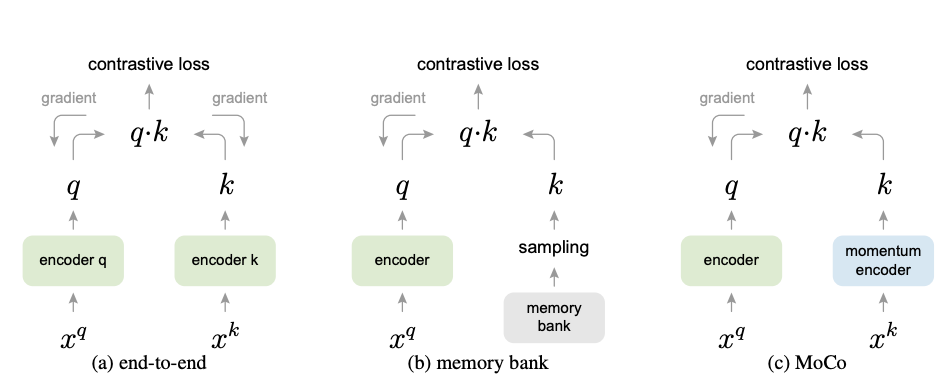
\includegraphics[width=\textwidth, height=5cm, natwidth=474, natheight=193]{Mal/momentum1.jpg}
  \caption{Концептуальне порівняння трьох контрастивних механізмів втрат.}
  \label{fig:momentum1}
\end{figure}

Оновлення end-to-end шляхом зворотного розповсюдження є природним механізмом. Він використовує зразки в поточній міні-партії як словник, тому ключі послідовно кодуються (тим самим набором параметрів кодера). Але розмір словника поєднується з міні-пакетним розміром, обмеженим обсягом пам'яті графічного процесора. Це також кидається виклик великій міні-пакетній оптимізації. Деякі останні методи засновані на завданнях підтексту, керованих місцевими позиціями, де розмір словника може бути збільшений на кілька позицій. Але для цих завдань-претекстів можуть знадобитися спеціальні мережеві конструкції, такі як патчіфікація вводу або налаштування сприйнятливого розміру поля, що може ускладнити перенесення цих мереж на подальші завдання [5].

Іншим механізмом є підхід банк пам'яті (memory bank). Банк пам'яті складається з подань усіх зразків у наборі даних. Словник для кожної міні-партії вибірково вибирається з банку пам'яті без зворотного розповсюдження, тому він може підтримувати великий розмір словника. Однак представлення вибірки в банку пам'яті було оновлено, коли її востаннє бачили, тому вибіркові ключі, по суті, стосуються кодерів на декількох різних етапах протягом усієї минулої епохи і, отже, менш послідовні. Оновлення імпульсу приймається на банку пам'яті. Її імпульс оновлення подається на поданнях того самого зразка, а не на кодері. Це оновлення імпульсу не має значення для нашого методу, оскільки MoCo не відстежує кожен зразок. Більше того, наш метод є більш ефективним в пам’яті, і його можна навчити на мільярдних даних, що може бути важко для банку пам'яті [5].

Порівняльне навчання може працювати з різними попередніми задачами.

Можна розглянути запит і ключ як позитивну пару, якщо вони походять з одного зображення, а в іншому $-$ як негативну пару вибірки. Візьмемо два випадкові «види» одного і того ж зображення під час випадкового збільшення даних, щоб сформувати позитивну пару. Запити та ключі кодуються відповідними кодерами $f_{q}$ та $f_{k}$. Кодером може бути будь-яка згорткова нейронна мережа.

Алгоритм Momentum Contrast для попередньої задачі можна реалізовувати по-різному. Наприклад: адаптувати нейронну мережу ResNet як кодер, чий останній повністю підключений шар (після загального середнього об'єднання) має вихід з фіксованим розміром (128-D). Цей вихідний вектор нормується за його L2-нормою. Це представлення запиту або ключа. Після чого потрібно обрати значення для аргументу $\tau$ з \ref{eq:infonce_simple}. Далі наведено параметр збільшення даних: обрізання $224 \times 224$ пікселів береться із зображення випадкового розміру, а потім піддається випадковому коливанню кольорів, випадковому горизонтальному перевертанню та випадковому перетворенню шкал сірого.

Обидва кодери $f_{q}$ і $f_{k}$ використовують пакетну нормалізацію (Batch Normalization, BN), як у стандартному ResNet. Можна показати, що використання BN заважає моделі засвоїти хороші уявлення.

Цю проблему можливо вирішити за допомогою тасування BN. Можна тренувати модель з декількома графічними процесорами та виконуввати BN на зразках незалежно для кожного графічного процесора (як це робиться у звичайній практиці). Для кодера ключів $f_{k}$ перемішується порядок зразків у поточній міні-партії перед розподілом між графічними процесорами (і перемішується назад після кодування). Порядок вибірки міні-партії для кодера запиту $f_{q}$ не змінюється. Це гарантує, що статистична інформація про партії, яка використовується для обчислення запиту, та її позитивний ключ надходять із двох різних підмножин. Це ефективно вирішує проблему дозволяє тренуванню принести користь від BN.

Використання перемішаного BN може стати у нагоді також у end-to-end оновленні. Це не має значення для банку пам'яті, який не страждає від цієї проблеми, оскільки позитивні ключі були від різних міні-пакетів у минулому.

\subsection{Висновки за розділом}

Порівняльне навчання $-$ це техніка машинного навчання, яка використовується для вивчення загальних особливостей набору даних без міток, навчаючи моделі, які точки даних подібні чи різні [6].

В результаті огляду літературних джерел для аналізу були обрані алгоритми Deep InfoMax (DIM) та Momentum Contrast (MoCo).

%\newpage
%%\section{Практична реалізація}
\section{ПРАКТИЧНА РЕАЛІЗАЦІЯ}

Даний розділ присвячується аналізу часового ряду тестувальної системи DOTS за допомогою мови програмування Python. 

Python $-$ це легка в освоєнні, потужна мова програмування. Він має ефективні структури даних високого рівня і простий, але ефективний підхід до об'єктно-орієнтованого програмування [10].

Python став загальноприйнятою мовою програмування для багатьох сфер застосування науки про дані. Дана мова програмування поєднує в собі міць мов програмування з простотою використання предметно орієнтованих скриптових мов типу MATLAB або R. 

В Python є бібліотеки для завантаження даних, візуалізації, статистичних обчислень, обробки природної мови, обробки зображень і багато чого іншого [11].

Також використовувався фреймфорк Anaconda. Це безкоштовний, включаючи комерційне використання, і готовий до використання в середовищі підприємства дистрибутив Python, який об'єднує всі ключові бібліотеки Python, необхідні для роботи в області науки про дані, математики та розробки, в одному зручному для користувача крос-платформенном дистрибутиві [12].

Для завантаження даних використовувалась бібліотека pandas. Бібліотека pandas надає структури даних і функції, покликані зробити роботу зі структурованими даними простим, швидким та вислови тельним справою. Це один з основних компонентів, що перетворюють Python в потужний інструмент продуктивного аналізу даних [13].

Також використовувалась бібліотека NumPy. NumPy є основним пакетом для наукових обчислень з Python [14].

\subsection{Підготування вхідних даних}

База даних тестувальної системи DOTS зберігається у форматі SQL-таблиць. В таблицях є спецільні символи, які не дозволяють використовувати таблицю. Після видалення цих символів, можна завантажити таблицю, яка має структуру наведену у рис. \ref{fig:DOTS}.

\vspace{1em}

\begin{figure}[h]
  \includegraphics[width=\textwidth, height=3cm, natwidth=1227, natheight=187]{DOTS.jpg}
  \caption{Структура бази даних тестувальної системи DOTS}
  \label{fig:DOTS}
\end{figure}

В базі даних є колонка $posted\_time$ $-$ це ціле число, яке відображає кількість мілісекунд від першого січня 1980 року. З циих чисел можна отримати дату відправлення до тестувальної системи. Після угрупування по датам отримуємо часовий ряд, наведений у рис. \ref{fig:TimeSeries}.


%Часовий ряд тестувальної системи DOTS має наступну структуру: в кожен день є певне ціле число відправлень, саме з цих чисел складається ряд. Часовий ряд наведено у рис. \ref{fig:TimeSeries}.

\vspace{1em}

\begin{figure}[h]
  \includegraphics[width=\textwidth, height=7cm, natwidth=854, natheight=476]{TimeSeries.jpg}
  \caption{Часовий ряд тестувальної системи DOTS}
  \label{fig:TimeSeries}
\end{figure}

Задля перевірки роботи алгоритму, часовий ряд було розділено на два ряди: тренувальний, та тестувальний. Будуть розглядати тренувальні ряди, які складають $90\%$ та $80\%$ від початкового, щоб побачити можливості алгоритмів для прогнозів разної тривалості.

\subsection{Аналіз та прогноз часового ряду за допомогою моделі ARIMA}
%\subsection{Аналіз та прогноз часового ряду з використанням моделі ARIMA}

У першому випадку, тренувальний ряд буде складати $90\%$ від початкового. У такому разі найбільш оптимальні параметри моделі ARIMA дорівнюють: $p = 6$, $d = 2$, $q = 4$. Результат прогнозування можна побачити на рис. \ref{fig:ARIMA90}.

\vspace{1em}

\begin{figure}[h]
  \includegraphics[width=\textwidth, height=7cm, natwidth=846, natheight=440]{ARIMA90.jpg}
  \caption{Порівняння оригінального та зпрогнозованого рядів}
  \label{fig:ARIMA90}
\end{figure}

%У табл. \ref{tab:ARIMA90} наведені параметри моделі та їхні до    вірчі інтервали.

Середня абсолютна процентна похибка (MAPE) дорівнює $17,84\%$, що є добрим прогнозом. У табл. \ref{tab:ARIMA90} наведені параметри моделі та їхні довірчі інтервали.

\begin{table}[h]
\caption{Довірні інтервали параметрів моделі}\label{tab:ARIMA90}
\begin{tabular}{|c|m{0.4\textwidth}|}
\hline
Параметр моделі & Довірчий інтервал \\
		\hlinewd{2pt}
$\alpha_{1} = -0,85$ & $-1,08 < -0,85 < -0,62$ \\
\hline
$\alpha_{2} = -0,93$ & $-1,13 < -0,93 < -0,72$ \\
\hline
$\alpha_{3} = -1,25$ & $-1,48 < -1,25 < -1,03$ \\
\hline
$\alpha_{4} = -0,94$ & $-1,14 < -0,94 < -0,75$ \\
\hline
$\alpha_{5} = -0,64$ & $-0,85 < -0,64 < -0,43$ \\
\hline
$\alpha_{6} = -0,45$ & $-0,62 < -0,45 < -0,28$ \\
\hline
$\theta_{1} = -0,98$ & $-1,12 < -0,98 < -0,84$ \\
\hline
$\theta_{2} = 0,34$ & $-0,04 < 0,34 < 0,65$ \\
\hline
$\theta_{3} = 0.45$ & $0.06 < 0.45 < 0.83$ \\
\hline
$\theta_{4} = -0,80$ & $-1,05 < -0,80 < -0,63$ \\
\hline
\end{tabular}
\end{table}

У випадку, коли тренувальний ряд дорівнює $80\%$ від початкового, то можемо бачити результати на рис. \ref{fig:ARIMA80}.

\newpage

\vspace{1em}

\begin{figure}[h]
  \includegraphics[width=\textwidth, height=7cm, natwidth=843, natheight=448]{ARIMA80.jpg}
  \caption{Порівняння оригінального та зпрогнозованого рядів}
  \label{fig:ARIMA80}
\end{figure}

Середня абсолютна процентна похибка (MAPE) дорівнює $45,94\%$, що є добрим прогнозом. У табл. \ref{tab:ARIMA80} наведені параметри моделі та їхні довірчі інтервали.

\begin{table}[h]
\caption{Довірні інтервали параметрів моделі}\label{tab:ARIMA80}
\begin{tabular}{|c|m{0.4\textwidth}|}
\hline
Параметр моделі & Довірчий інтервал \\
		\hlinewd{2pt}
$\alpha_{1} = -0,99$ & $-1,22 < -0,99 < -0,75$ \\
\hline
$\alpha_{2} = -1,08$ & $-1,31 < -1,08 < -0,85$ \\
\hline
$\alpha_{3} = -1,39$ & $-1,63 < -1,39 < -1,14$ \\
\hline
$\alpha_{4} = -1,08$ & $-1,30 < -1,08 < -0,85$ \\
\hline
$\alpha_{5} = -0,75$ & $-0,97 < -0,75 < -0,52$ \\
\hline
$\alpha_{6} = -0,52$ & $-0,69 < -0,52 < -0,34$ \\
\hline
$\theta_{1} = -0,88$ & $-1,11 < -0,88 < -0,64$ \\
\hline
$\theta_{2} = 0,28$ & $-0,08 < 0,28 < 0,64$ \\
\hline
$\theta_{3} = 0,43$ & $0.04 < 0.43 < 0.82$ \\
\hline
$\theta_{4} = -0,83$ & $-1,04 < -0,83 < -0,62$ \\
\hline
\end{tabular}
\end{table}

\subsection{Аналіз та прогноз часового ряду за допомогою алгоритму SSA}

У випадку алгоритму SSA будемо тестувати різні довжини вікон.

Якщо довжина вікна дорівнює $10$, та тренувальний ряд складає $90\%$ оригінального, то отримуємо результати приведені у рис. \ref{fig:SSA9010}.

\vspace{1em}

\begin{figure}[h]
  \includegraphics[width=\textwidth, height=6cm, natwidth=872, natheight=447]{SSA9010.jpg}
  \caption{Порівняння оригінального та зпрогнозованого рядів}
  \label{fig:SSA9010}
\end{figure}

В такому випадку $\text{MAPE} = 37,04\%$.

Якщо довжина вікна дорівнює $17$, та тренувальний ряд складає $90\%$ оригінального, то отримуємо результати приведені у рис. \ref{fig:SSA9016}.

\vspace{1em}

\begin{figure}[h]
  \includegraphics[width=\textwidth, height=7cm, natwidth=880, natheight=447]{SSA9016.jpg}
  \caption{Порівняння оригінального та зпрогнозованого рядів}
  \label{fig:SSA9016}
\end{figure}

1-а власна трійка приведена на рис. \ref{fig:Trend90} відповідає тренду:

\newpage

\vspace{1em}

\begin{figure}[h]
  \includegraphics[width=\textwidth, height=7cm, natwidth=822, natheight=408]{Trend90.jpg}
  \caption{Трендова складова}
  \label{fig:Trend90}
\end{figure}

2-а власна трійка є сезонною складовою. Її приведено на рис. \ref{fig:Cyclic190}.

\vspace{1em}

\begin{figure}[h]
  \includegraphics[width=\textwidth, height=7cm, natwidth=817, natheight=410]{Cyclic190.jpg}
  \caption{Перша сезонна складова}
  \label{fig:Cyclic190}
\end{figure}

Як можна побачити з графіку, 3-я власна трійка є також сезонною складовою. Її приведено на рис. \ref{fig:Cyclic290}.

\newpage

\vspace{1em}

\begin{figure}[h]
  \includegraphics[width=\textwidth, height=7cm, natwidth=820, natheight=411]{Cyclic290.jpg}
  \caption{Друга сезонна складова}
  \label{fig:Cyclic290}
\end{figure}


Якщо подивитися на двовимірну діаграму між 14 та 15 власними трійками, приведену на рис. \ref{fig:Diag90}, можна зробити висновок, що всі власні трійки після 14 відповідають за шумові процеси і їх можна не розглядати.


\vspace{1em}

\begin{figure}[h]
  \includegraphics[width=\textwidth, height=7cm, natwidth=837, natheight=422]{Diag90.jpg}
  \caption{Двовимірна діаграма 14 і 15 власних трійок}
  \label{fig:Diag90}
\end{figure}

В такому випадку $\text{MAPE} = 29,68\%$. Експерементальним шляхом було визначено, що дане значення є оптимальним.

Якщо довжина вікна дорівнює $10$, та тренувальний ряд складає $80\%$ оригінального, то отримуємо результати приведені у рис. \ref{fig:SSA8010}.

\newpage

\vspace{1em}

\begin{figure}[h]
  \includegraphics[width=\textwidth, height=7cm, natwidth=876, natheight=436]{SSA8010.jpg}
  \caption{Порівняння оригінального та зпрогнозованого рядів}
  \label{fig:SSA8010}
\end{figure}

В такому випадку $\text{MAPE} = 47.59\%$.

Якщо довжина вікна дорівнює $11$, та тренувальний ряд складає $80\%$ оригінального, то отримуємо результати приведені у рис. \ref{fig:SSA8011}.

\begin{figure}[h]
  \includegraphics[width=\textwidth, height=7cm, natwidth=868, natheight=435]{SSA8011.jpg}
  \caption{Порівняння оригінального та зпрогнозованого рядів}
  \label{fig:SSA8011}
\end{figure}

В такому випадку $\text{MAPE} = 40.22\%$. Експерементальним шляхом було визначено, що дане значення є оптимальним.

\subsection{Висновки за розділом}

В даному розділі була продемонстрована робота алгоритмів ARIMA та SSA. БУли реалізовані програми мовою програмування Python за допомогою спеціальних бібліотек для аналізу даних та програмного фреймворку Anaconda. 

Як видно з результатів, модель ARIMA дає якісніший короткотривалий прогноз, в той час як алгоритм SSA дає більш якісний довготривалий прогноз.

Можна також комбінувати ці моделі, щоб отримати більш якісний прогноз.

%\newpage
%\section{Економічне обґрунтування}
\section{ЕКОНОМІЧНЕ ОБҐРУНТУВАННЯ}

Темою дипломної бакалаврської роботи є «Розробка методів представлення візуальної інформації за допомогою методів самонавчання та contrastive learning». В процесі роботи була розглянута необхідна теорія, а також був створений програмний продукт. Важливою частиною дипломної роботи є економічне обгрунтування.

\subsection{Розрахунок кошторису витрат на проведення й впровадження результатів науково-дослідної роботи}
Виконання наукових дослiджень, а також впровадження результатiв НДР вимагає певних витрат, якi необхiдно розглядати як додатковi капiталовкладення. Витрати на проведення й впровадження результатiв НДР вiдносяться до виробничих витрат. 

Як правило, всi витрати документально оформляються у виглядi кошторису. Основними статтями кошторису витрат є заробiтна плата, нарахування на заробiтну плату, вартiсть електроенергiї (технологiчна й освiтлювальної), вартiсть оренди примiщення, амортизацiйнi вiдрахування на обчислювальну технiку, вартiсть впровадження й освоєння результатiв НДР i плановi накопичення.

\subsubsection{Розрахунок фонду заробітної плати виконавців}
Розрахунок фонду заробiтної плати виконавцiв проводиться виходячи зi штатного розкладу й зайнятостi виконавцiв у данiй НДР.
Виконавцями даної НДР є керівник дипломної роботи, консультанти частини економічного обґрунтування й частини охорони праці дипломної роботи, а також студент. Штатний розклад приведено у табл. \ref{tab:staff}.

\newpage

\begin{table}
	\captionstyle{ \raggedright}
	\caption{Штатний розклад}\label{tab:staff}
	\begin{tabular}{| p{0.20\textwidth} | p{0.12\textwidth} | p{0.12\textwidth} | p{0.14\textwidth} | p{0.14\textwidth} | p{0.14\textwidth} |}
		\hline
		Посада & Кількість виконавців & Час зайнятості, міс & Коефіціент трудової участі & Оклад на місяць, грн & Заробітна плата, $\text{Зп}_{\text{оклад}}$, грн \\
		\hlinewd{2pt}
		1 Керівник роботи, старший викладач & 1 & 4 & 0,075 & 7000 & 2100\\
		\hline
		2 Консультант частини економічного обгрунтування, професор & 1 & 4 & 0,005 & 10000 & 200\\
		\hline
		3 Консультант частини охорони праці, доцент & 1 & 4 & 0,005 & 8000 & 160\\
		\hline
		4 Консультант частини цивільного захисту, старший викладач & 1 & 4 & 0,005 & 7000 & 140\\
		\hline
		5 Виконавець, студент & 1 & 4 & 1 & 1600 & 6400\\
		\hline
	\end{tabular}
\end{table}

Заробітна плата виконавців НДР складається з основної заробітної плати й різних доплат до неї:

\begin{equation}\label{eq:zp}
\text{Зп} = \text{Зп}_{\text{осн}} + \text{Зп}_{\text{д}},
\end{equation}

\noindent де $\text{Зп}_{\text{осн}}$ $-$ основна заробітна плата; \newline 
\hspace*{15pt} $\text{Зп}_{\text{д}}$ $-$ доплати до заробітної плати.


\begin{equation}
\text{Зп}_{\text{осн}} = \text{Зп}_{\text{оклад}} + \text{Зп}_{\text{прем}},
\end{equation}

\noindent де $\text{Зп}_{\text{оклад}}$ $-$ розмір заробітної плати за штатним розкладом; \newline
\hspace*{15pt} $\text{Зп}_{\text{прем}}$ $-$ розмір премій. 

\begin{equation}
\text{Зп}_{\text{прем}} = \text{К}_{\text{прем}} \cdot \text{Зп}_{\text{оклад}},
\end{equation}

\noindent де $\text{К}_{\text{прем}}$ $-$ коефіціент преміювання, $\text{К}_{\text{прем}} = 0,1$;

\begin{equation}
\text{Зп}_{\text{д}} = \text{К}_{\text{д}} \cdot \text{Зп}_{\text{осн}},
\end{equation}

\noindent де $\text{К}_{\text{д}}$ $-$ коефіцієнт доплат заробітної плати, $\text{К}_{\text{д}} = 0,1$. 

\vspace{1.5em}

Розрахуємо заробітню плату виконавців НДР.

Керівник дипломної роботи:

\[
\text{Зп} = 2100 + 2100 \cdot 0,1 + 0,1 \cdot (2100 + 2100 \cdot 0,1) = 1220,80 \, \text{грн}.
\]

\vspace{1.5em}

Консультант частини економічного обгрунтування:

\[
\text{Зп} = 250 + 250 \cdot 0,12 + 0,09 \cdot (250 + 250 \cdot 0,12) = 305,20 \, \text{грн}.
\]

\vspace{1.5em}

Консультант частини охорони праці:

\[
\text{Зп} = 200 + 200 \cdot 0,12 + 0,09 \cdot (200 + 200 \cdot 0,12) = 244,16 \, \text{грн}.
\]

\vspace{1.5em}

Консультант частини цивільного захисту:

\[
\text{Зп} = 200 + 200 \cdot 0,12 + 0,09 \cdot (200 + 200 \cdot 0,12) = 244,16 \, \text{грн}.
\]

\vspace{1.5em}

Фонд заробiтної плати виконавцiв складе:

\[
\text{Зп}_{\text{заг}} = 1220,80 + 305,20 + 244,16 + 7000,00 = 8770,16 \, \text{грн}.
\]

\vspace{1.5em}

Всього витрати на заробiтну плату склали 8770,16 грн.

\subsubsection{Відрахування на соціальне страхування}

Відрахування на соціальне страхування й інші відрахування розраховуються на підставі отриманого значення фонду заробітної плати:

\begin{equation}\label{eq:soc}
\text{Від} = \text{К}_{\text{від}} \cdot \text{Зп},
\end{equation}


\noindent де $\text{К}_{\text{від}}$ $-$ коефіцієнт нарахувань на фонд заробітної плати приймається в розмірі $0,362$.

\[
\text{Від} = 0,362 \cdot 1770,16 = 640,79 \, \text{грн}.
\]

\vspace{1.5em}

\subsubsection{Розрахунок технологічної електроенергії}

Розрахунок технологічної електроенергії проводиться виходячи із завантаження устаткування, що використовується під час проведення НДР (ЕОМ, принтер, сканер і ін.), по формулі (\ref{eq:texenergy}):

\begin{equation}\label{eq:texenergy}
\text{Е}_{\text{тех}} = P \sum_{i=1}^{N}\text{П}_{i}T_{i}
\end{equation}

\noindent де $P$ $-$ тариф на електроенергію, $P = 1,7808 \, \text{грн}/\text{кВт}$; \newline
\hspace*{15pt} $\text{П}_{i}$ $-$ споживана потужність $i$-ої одиниці встаткування, для комп'ютера $\text{П}_{i} = 0,3 \, \text{кВт}/\text{год}$;\newline
\hspace*{15pt} $T_{i}$ $-$ час роботи $i$-ої одиничі встаткування, $T_{1} = 336 \, \text{год}$.

\[
\text{Е}_{\text{тех}} = 1,7808 \cdot 0,3 \cdot 336 = 179,50 \, \text{грн}.
\]

\vspace{1.5em}

\subsubsection{Розрахунок електроенергії, що витрачається на освітлення}

Розрахунок електроенергії, що витрачається на освітлення, виконується виходячи з норм охорони праці по освітленню робочих місць та розраховується наступним чином:

\begin{equation}\label{eq:osv}
\text{Е}_{\text{осв}} = P \cdot N_{\text{л}} \cdot \text{П}_{\text{л}} \cdot T,
\end{equation}

\noindent де $P$ $-$ тариф на електроенергію, $P = 1,7808 \, \text{грн}/\text{кВт}$; \newline
\hspace*{15pt}$N_{\text{л}}$ $-$ кількість ламп, $N_{\text{л}} = 2$;\newline
\hspace*{15pt}$\text{П}_{\text{л}}$ $-$ споживана потужність однієї лампи, $\text{П}_{\text{л}} = 0,1 \, \text{кВт}/\text{год}$;\newline
\hspace*{15pt}$T$ $-$ час роботи ламп для освітлення, $T = 169 \, \text{год}$.

\[
\text{Е}_{\text{осв}} = 1,7808 \cdot 2 \cdot 0,1 \cdot 169 = 60,19 \, \text{грн}.
\]

\vspace{1.5em}

\subsubsection{Амортизаційні відрахування на устаткування}

Амортизацiйнi витрати розраховуються виходячи з формули (\ref{eq:amort}):

\begin{equation}\label{eq:amort}
A = \frac{a_{\text{ЕОМ}}}{12}\sum_{i=1}^{N}\text{ЗВ}_{i} \cdot T_{i},
\end{equation}

\noindent де $a_{\text{ЕОМ}}$ $-$ річна норма амортизації, прийнята в розмірі $ 26 \, \%$ залишкової вартості устаткування;\newline
\hspace*{23pt}$\text{ЗВ}_{i}$ $-$ залишкова вартість $i$-ої одиниці устаткування, $\text{ЗВ}_{1} = 4739,78 \, \text{грн}$;\newline
\hspace*{23pt}$T_{i}$ $-$ час використання $i$-ої одиниці устаткування $T_{1} = 3,5 \, \text{міс}$.

\[
A = \frac{0,26}{12} \cdot 4739,78 \cdot 3,5 = 359,43 \, \text{грн}.
\]

\vspace{1.5em}

\subsubsection{Вартість оренди приміщення}

Витрати на оренду примiщення розраховуються виходячи з формули (\ref{eq:orenda}):

\begin{equation}\label{eq:orenda}
\text{Д} = \text{К}_{\text{а}} \cdot S \cdot P \cdot T_{OP},
\end{equation}

\noindent де $\text{К}_{\text{а}}$ $-$ коефіцієнт, що враховує податок на майно, $\text{К}_{\text{а}} = 1,25$;\newline
\hspace*{19pt}$S$ $-$ площа приміщення, де проводилася НДР, $S = 10 \, \text{м}^{2}$;\newline
\hspace*{19pt}$P$ $-$ вартість оренди одного квадратного метра приміщення, $P = 195 \, \text{грн}/\text{міс}$;\newline
\hspace*{19pt}$T_{OP}$ $-$ строк оренди, $T_{OP} = 5 \, \text{міс}$.

\[
\text{Д} = 1,25 \cdot 10 \cdot 195 \cdot 5 = 12187,50 \, \text{грн}.
\]

\vspace{1.5em}

\subsubsection{Інші витрати}

Інші витрати (опалення, робота кондиціонера й ін.), згідно з формулою (\ref{eq:inshi}), приймаються в розмірі $7,5\%$ від вартості оренди приміщення. 

\begin{equation}\label{eq:inshi}
\text{З}_{\text{ін}} = \text{Д} \cdot \text{К}_{\text{ін}} = 12187,50 \cdot 0,075 = 914,06 \, \text{грн}. 
\end{equation}

\vspace{1.5em}

\subsubsection{Вартість впровадження й освоєння результатів НДР}

Результатом НДР є система, яка дослілджує та аналізує динаміку відправлень рішень до тестувальної системи. Для використання цієї системи необхідно впровадити та освоїти програми у аналітичних відділах.

При впровадженнi та освоєннi результатiв НДР необхiдно залучити хоча б одного асистента кафедри в науково дослiдному iнститутi з вiдповiдної спецiальностi. Заробiтна плата становить 5000 грн на мiсяць в середньому. На впровадження необхiдно не менше мiсяця. У пiдсумку вартiсть впровадження та освоєння результатiв НДР складе $5000$ грн.

\subsubsection{Витрати на проведення НДР}

Витрати на проведення НДР, згідно з формулою (\ref{eq:vitraty}), являють собою суму витрат по окремих статтях:

\begin{equation}\label{eq:vitraty}
\text{З} = \text{Зп} + \text{Від} + \text{Е}_{\text{тех}} + \text{Е}_{\text{осв}} + \text{А} + \text{Д} + \text{З}_{\text{ін}} + \text{В}_{\text{вп}},
\end{equation}

\noindent де $\text{З}_{\text{ін}}$ $-$ інші витрати; \newline
\hspace*{15pt} $ \text{В}_{\text{вп}}$ $-$ вартість впровадження й освоєння результатів НДР.

Таким чином, сукупнi витрати складають:

\begin{eqnarray*}
\text{З} = 8770,16 + 640,79 + 179,50 + 60,19 + 359,43 + \\ + 12187,50 + 914,06 + 5000  = 28111,63 \, \text{грн}.
\end{eqnarray*}

\vspace{1.5em}

\subsubsection{Планові накопичення}

Планові накопичення обираються в розмірі $30\%$ від витрат на проведення НДР та наведені у формулі (\ref{eq:plan}).

\begin{equation}\label{eq:plan}
\text{ПН} = 0,3 \cdot 28111,63 = 8433,48 \, \text{грн}.
\end{equation}

\vspace{1.5em}

\subsubsection{Кошторис витрат на проведення НДР}

Кошторис витрат на проведення НДР є сумою витрат на проведення НДР і планових накопичень. Результати розрахунку кошторису витрат представлені у табл. \ref{tab:sumNDR}.

\begin{table}[hbt]
	\captionstyle{ \raggedright}
	\caption{Кошторис витрат на проведення НДР}\label{tab:sumNDR}
	%\centering
	\begin{tabular}{|p{0.65\textwidth}|p{0.15\textwidth}|}
		\hline
		Стаття витрат & Сума, грн \\
		\hlinewd{2pt}
		1 Заробiтна плата & 8770,16 \\
		\hline
		2 Вiдрахування на соцiальне страхування & 640,79 \\
		\hline
		3 Технологiчна електроенергiя & 179,50 \\
		\hline
		4 Електроенергiя на освiтлення & 60,19 \\
		\hline
		5 Амортизацiйнi вiдрахування на устаткування & 359,43 \\
		\hline
		6 Вартiсть оренди примiщення & 12187,50 \\
		\hline
		7 Iншi витрати & 914,06 \\
		\hline
		8 Вартiсть впровадження та освоєння НДР & 5000 \\
		\hline
		9 Разом витрат & 28111,63 \\
		\hline
		10 Плановi накопичення & 8433,48 \\
		\hline
		11 Усього кошторис витрат на НДР & 36545,11 \\
		\hline
	\end{tabular}
\end{table}

\subsection{Висновки за розділом}

В процесі роботи над економічною частиною НДР було проведено ознайомлення з методикою складання кошторису витрат на НДР та подальший його розрахунок за основними статтями: витрати на заробiтну платню виконавцiв дипломної роботи, витрати на електроенергiю, амортизацiйнi вiдрахування, вiдрахування на соцiальне страхування, оренду примiщення i плановi накопичення. За результатами проведених розрахункiв кошторис склав $36545,11$ грн.

\newpage
%%\section{Охорона праці і навколишнього середовища}
\section{ОХОРОНА ПРАЦІ І НАВКОЛИШНЬОГО СЕРЕДОВИЩА}

\subsection{Аналіз умов праці на робочому місці}

Розділ виконано для етапу розробки на ЕОМ системи створення програмного комплексу для аналізу роботи алгоритмів порівняльного навчання.

Робота виконувалась на кафедрі «Комп’ютерної математики та аналізу даних» НТУ «ХПІ», яка розташована на другому поверсі семи поверхової будівлі.

Обладнання, приміщення і режим праці користувача повинні відповідати вимогам наступних нормативно–технічних документів:

\begin{enumerate}
	\item НПАОП 0.00-7.15-18.\hfill Вимоги\hfill щодо\hfill безпеки\hfill та\hfill захисту\hfill здоров’я\newline \hspace*{-20mm} працівників під час роботи з екранними пристроями.
	\item ДСанПіН 3.3.2.007-98.\hfill Державні\hfill санітарні\hfill правила\hfill і\hfill норми\newline \hspace*{-20mm} роботи\hfill з\hfill візуальними\hfill дисплейними\hfill терміналами\hfill електронно-\newline \hspace*{-18mm}обчислювальних машин. 
	\item ДСТУ Б В.1.1-36:2016.\hfill Визначення\hfill категорій\hfill приміщень,\hfill будинків\newline \hspace*{-18mm} та зовнішніх установок за вибухопожежною та пожежною небезпекою. 
	\item ДБН В.1.1-7-2016.\hfill Пожежна\hfill безпека\hfill об’єктів\hfill будівництва.\newline \hspace*{-18mm} Загальні вимоги. 
	\item ДСН 3.3.6.042-99.\hfill Санітарні\hfill норми\hfill мікроклімату\hfill виробничих\newline \hspace*{-18mm} приміщень.
	\item ДБН В.2.5-67:2013. Опалення, вентиляція та кондиціонування.
	\item ДБН В.2.5-28-2018. Природне та штучне освітлення.
	\item ДСН 3.3.6.037-99.\hfill Санітарні\hfill норми\hfill виробничого\hfill шуму,\hfill ультразвуку\newline \hspace*{-18mm} та інфразвуку.
	\item ДСН 3.3.6.039-99.\hfill Санітарні\hfill норми\hfill виробничої\hfill загальної\newline \hspace*{-18mm} та локальної вібрації.
	\item ПУЕ. Правила улаштування електроустановок. 
	\item НПАОП 40.1-1.32-01.\hfill Правила\hfill будови\hfill електроустановок.\newline \hspace*{-18mm} Електрообладнання спеціальних установок.
	\item ДСТУ ГОСТ 7237:2011.\hfill Електробезпека.\hfill Загальні\hfill вимоги\newline \hspace*{-18mm} та номенклатура видів захисту.
	\item ГОСТ 14254-96. Степени защиты, обеспечиваемые оболочками.
	\item НАПБ А.01.001-2014. Правила пожежної безпеки в Україні.
	\item ДСТУ БВ.2.5-38:2008.\hfill Інженерне\hfill обладнання\hfill будинків\hfill і\hfill споруд.\newline \hspace*{-18mm} Улаштування блискавка захисту будівель і споруд (IEC 62305:2006, NEQ).
	\item НАПБ Б.06.004-2005.\hfill Перелік\hfill однотипних\hfill за\hfill призначенням\newline \hspace*{-18mm} об’єктів,\hfill які\hfill підлягають\hfill обладнанню\hfill автоматичними\hfill установками\hfill пожежа\newline \hspace*{-18mm} гасіння та пожежної сигналізації.
	\item ГН 3.3.5-8.6.6.1-2014. \hfill Гігієнічна\hfill класифікація\hfill праці\hfill за\newline \hspace*{-18mm} показниками\hfill шкідливості\hfill та\hfill небезпечності\hfill факторів\hfill виробничого\newline \hspace*{-18mm} середовища, важкості та напруженості трудового процесу.
\end{enumerate}

\subsubsection{Загальна характеристика виробничого приміщення}

Загальна характеристика виробничого приміщення, в якому виконувалась робота, приведена у таблицях \ref{tab:work1-1}-\ref{tab:work1-3}.

\begin{table}[h]
	\captionstyle{ \raggedright}
	\caption{Загальна характеристика виробничого приміщення}\label{tab:work1-1}
	%\centering
	\begin{tabular}{|m{0.18\textwidth}|m{0.2\textwidth}|m{0.185\textwidth}|m{0.16\textwidth}|m{0.175\textwidth}|}
		\hline
		Найменування показника& Характеристика показника & Обґрунтування вибору значення показника & Документ, що регламентує цей показник & Примітка \\
		\hlinewd{2pt}
		1. Розміри приміщення (м); & $3.5 \times 4$ & \multirow{2}{*}{\parbox[t]{0.18\textwidth}{на одне р. м. з ЕОМ не менше 6.0 $\text{м}^{2}$ площі }} & \multirow{2}{*}{\parbox[t]{0.18\textwidth}{ДСанПіН \\3.3.2-007-98}} & \multirow{2}{*}{\parbox[t]{0.18\textwidth}{7 $\text{м}^{2}$ на одне р. м. з ЕОМ, що відповідає нормі}} \\
		\cline{1-2}
		2. Кількість робочих місць (р.м.) & 2 & & & \\ %[-0.3em]
		\hline
	\end{tabular}
\end{table}

%З характеристикою освітлення можна ознайомитись у таблиці \ref{tab:work1-2}.

\newpage

\begin{table}[h!]
	\captionstyle{ \raggedright}
	\caption{Характеристика освітлення}\label{tab:work1-2}
	%\centering
	\begin{tabular}{|m{0.18\textwidth}|m{0.2\textwidth}|m{0.185\textwidth}|m{0.16\textwidth}|m{0.175\textwidth}|}
		\hline
		Найменування показника& Характеристика показника & Обґрунтування вибору значення показника & Документ, що регламентує цей показник & Примітка \\
		\hlinewd{2pt}
		\multirow{2}{*}{\parbox[t]{0.18\textwidth}{1. Природне освітлення, вікна виходять на схід}} & \multirow{2}{*}{\parbox[t]{0.18\textwidth}{бокове, одностороннє; азимут $90^{\degree}$}} & див. таблицю \ref{tab:work2-2} & ДБН В.2.5-28-18 &  \\
		\cline{3-5}
		& & КПО не нижче 1.5 \% & ДСанПіН 3.3.2-007-98 & для р. м. з ЕОМ \\ [2em]
		\hline
		\multirow{2}{*}{\parbox[t]{0.18\textwidth}{2. Штучне освітлення, кількість світильників N; джерела світла}} & \multirow{2}{*}{\parbox[t]{0.18\textwidth}{загальне рівномірне; N=10; люмінесцентні лампи}} & див. таблицю \ref{tab:work2-2} & ДБН В.2.5.-28-06 &  \\
		\cline{3-5}
		& & не нижче 300-500 лк & ДСанПіН 3.3.2-007-98 & для р. м. з ЕОМ \\ [3.5em]
		\hline
	\end{tabular}
\end{table}

%У таблиці \ref{tab:work1-4} з факторами пожежної безпеки.

%\newpage

\begin{table}[h!]
	\captionstyle{ \raggedright}
	\caption{Характеристика пожежної безпеки}\label{tab:work1-4}
	%\centering
	\begin{tabular}{|m{0.22\textwidth}|m{0.22\textwidth}|m{0.22\textwidth}|m{0.22\textwidth}|}
		\hline
		Найменування показника& Характеристика показника & Обґрунтування вибору значення показника & Документ, що регламентує цей показник \\
		\hlinewd{2pt}
		1. Категорія приміщення з вибухо–пожеже небезпеки & В & є тверді спаленні матеріали: папір, деревина тощо & ДСТУ Б В.1.1-36:2016 \\
		\hline
		2. Ступінь вогнестійкості будівельних конструкцій & ІІ & 5-и поверхова будівля; категорія В & ДБН В.1.1.7-2016 \\
		\hline
	\end{tabular}
\end{table}

%Характеристика електромережі представлена у таблиці \ref{tab:work1-3}.

\newpage

\begin{table}[h]
	\captionstyle{ \raggedright}
	\caption{Характеристика електронної мережі}\label{tab:work1-3}
	%\centering
	\begin{tabular}{|m{0.18\textwidth}|m{0.2\textwidth}|m{0.185\textwidth}|m{0.16\textwidth}|m{0.175\textwidth}|}
		\hline
		Найменування показника& Характеристика показника & Обґрунтування вибору значення показника & Документ, що регламентує цей показник & Примітка \\
		\hlinewd{2pt}
		1. Характеристика трифазної електричної мережі & чотири провідна з глухо заземленою нейтраллю напругою 380/220 В, частотою 50 Гц & довгі кабельні мережі великої ємності & ПУЕ & \\
		\hline
		2. Клас приміщення за ступенем небезпеки ураження електрострумом & з підвищеною небезпекою & є можливість одночасного дотику до металоконструкцій будівлі, що мають з’єднання з землею, та до металевих корпусів ЕОМ & ПУЕ & необхідно передбачити заходи безпеки згідно вимог ПУЕ \\
		\hline
	\end{tabular}
\end{table}


\subsubsection{Небезпечні та шкідливі фактори}

Небезпечним називають виробничий фактор, вплив якого на організм працюючого у відповідних умовах праці може призвести до травм або іншого раптового, різкого погіршення стану здоров’я.

Шкідливим називають виробничий фактор, вплив якого на організм працюючого може призводити в певних умовах до захворювання або зниження рівня працездатності.

Згідно з державним стандартом шкідливі і небезпечні фактори по природі їх впливу поділяються на фізичні, хімічні, біологічні та психофізіологічні.

Однією із основних цілей охорони праці на підприємстві є оцінка обстановки та характеристик трудового процесу в частині його впливу на здоров’я і життя працівника.

У таблиці \ref{tab:work2-1} надано перелік потенційних небезпечних факторів на робочому місці користувача ЕОМ з монітором на рідинних кристалах.

\begin{table}[hbt]
	\captionstyle{ \raggedright}
	\caption{Перелік потенційних небезпечних факторів на робочому місці користувача ЕОМ з ЖК монітором}\label{tab:work2-1}
	%\centering
	\begin{tabular}{|m{0.18\textwidth}|m{0.2\textwidth}|m{0.185\textwidth}|m{0.17\textwidth}|m{0.165\textwidth}|}
		\hline
		Назва фактора& Джерела виникнення& Умови роботи& Нормативні параметри, їх значення & Документ, що регламентує показник \\
		\hlinewd{2pt}
		Висока електрична напруга & мережа живлення устаткування & нормальний режим роботи & струм $Іh = 0,3$ мА; Напруга $U_\text{дот} < 2$ В & ДСТУ ГОСТ 12.1.038:08 \\
		\hline
	\end{tabular}
\end{table}

Таблиця \ref{tab:work2-2} показує типовий перелік потенційних шкідливих факторів.

\newpage

\begin{table}[hbt!]
	\captionstyle{ \raggedright}
	\caption{Перелік потенційних шкідливих факторів на робочому місці користувача ЕОМ з ЖК монітором}\label{tab:work2-2}
	%\centering
	\begin{tabular}{|m{0.18\textwidth}|m{0.2\textwidth}|m{0.185\textwidth}|m{0.17\textwidth}|m{0.165\textwidth}|}
		\hline
		Назва фактора& Джерела виникнення& Умови роботи& Нормативні параметри, їх значення & Документ, що регламентує показник \\
		\hlinewd{2pt}
		Несприятливе освітлення & стан систем природного та штучного освітлення & МРОР 0,3–0,5 мм; підрозряд «в», фон та контраст середні & КПО $D^{н}_{min} = 1,2 \, \%$; Освітленість $E_{min} = 300$ лк & ДБН В.2.5.–28–18 \\
		\hline
		\parbox[t]{0.18\textwidth}{Несприятли-\\вий мікроклімат: $t$, $\phi$, $v$} & стан систем опалення та вентиляції & категорія важкості робіт Іа; холодний період & $t$ $-$ $22–24 \, ^{\degree}C$; $\phi$ $-$ $40-60 \, \%$; $v$ $-$ не більше $0,1$ м/с & ДСН 3.3.6.042–99 \\
		\hline
		Підвищений рівень шуму & кондиціонери, кулери, системи освітлювання & творча діяльність, програмування & рівень звуку $L_{A} = 50 \, \text{дБА}$ & ДСН 3.3.6.037–99 \\
		\hline
		Вібрація & те ж саме & загальна технологічна, категорія 3, тип «в», умови комфорту & рівень віброшвидкості $L_{V} = 75 \, \text{дБ}$ & ДСТУ ГОСТ 12.1.012:08 ДСН 3.3.6.039–99 \\
		\hline
		\parbox[t]{0.18\textwidth}{Психо–фізіо-\\логічна перенапруга} & \parbox[t]{0.2\textwidth}{монотонність праці, стати-\\чність і незручність пози} & & 1 та 2 клас умов праці для напруженості & \parbox[t]{0.165\textwidth}{ГН 3.3.5–8.6.6.1-\\2002} \\
		\hline
	\end{tabular}
\end{table}

\newpage

\subsection{Захист від шкідливого впливу факторів виробничого середовища}

Підтримка оптимальних параметрів мікроклімату в робочій зоні здійснюється відповідно вимог ДБН В.2.5-67:2013 за допомогою кондиціонеру, який регулює температуру повітря. Передбачена можливість природнього провітрювання приміщення. У холодний період року проводиться опалення від центральної тепломережі.

Згідно ДСН 3.3.6.042-99, у приміщеннях із значними площами засклених поверхонь передбачаються заходи щодо захисту:

\begin{enumerate}
	\item від\hfill перегрівання\hfill при\hfill попаданні\hfill прямих\hfill сонячних\hfill променів\hfill в\newline \hspace*{-18mm} теплий\hfill період\hfill року\hfill (орієнтація\hfill віконних\hfill прорізів\hfill схід\hfill – захід,\newline \hspace*{-18mm} улаштування лоджій, жалюзі, сонцезахисних плівок та інше);
	\item від\hfill радіаційного\hfill охолодження $-$ в\hfill зимовий\hfill (використання\hfill стін\newline \hspace*{-18mm} певної товщини, подвійних стекол).
\end{enumerate}

Робочі місця повинні бути віддалені від стін на відстань не менше 1 м. 

Визначений в таблиці \ref{tab:work2-2} коефіцієнт природного освітлення реалізується через вікна визначеної площини, яка розраховується при проектуванні будівлі, а нормований показник штучного освітлення ($E_{min}$) реалізується шляхом встановлення визначеної кількості світильників і вибором потужності ламп в них.

Згідно вимог ДСанПіН 3.3.2.007-98, в разі штучного освітлення як джерела світла мають застосовуватись переважно люмінісцентні лампи типу ЛБ і світильники серії ЛПО3б із дзеркальними гратами, укомплектовані високочастотними пускорегулювальними апаратами (ВЧ ПРА).

Система загального освітлення має становити суцільні або преривчасті лінії світильників, розташовані збоку від робочих місць (переважно ліворуч), паралельно лінії зору працюючих. Слід передбачити обмеження прямої блискості від джерел природного та штучного освітлення та обмежувати відбиту блискість на робочих поверхнях. Необхідно чистити вікна і світильники не менше двох разів на рік та вчасно заміняти перегорілі лампи.

Заходи захисту від шуму та вібрації повинні відповідати вимогам ГОСТ 12.1.029-80 і ДСТУ ГОСТ 2656885:2009. Устаткування, що є джерелом шуму, слід розташовувати поза приміщенням для роботи з ЕОМ. Для забезпечення допустимих рівнів шуму у виробничих приміщеннях слід застосовувати засоби звукопоглинання, наприклад, перфоровані плити, панелі, підвісні стелі.

Як захист від шуму, який створюється вентиляторами системних блоків, використовується звукоізоляційний корпус. Вентилятор можна замінити на більш якісний або на мідні радіатори з водяним охолодженням. Крім того встановлюють перехідник з регулятором напруги і швидкості обертання процесорного кулеру, а при монтажі кулерів металеві гвинти заміняють гумовими пробками, що дозволяють ізолювати вентилятор від корпусу. Якщо принтер розташований на твердій поверхні, то для зменшення вібрації потрібно підстелити під нього щільний прогумований килимок.

\subsection{Електробезпека}

Персональна ЕОМ є однофазним споживачем електроенергії, який живиться від трифазної чотирьох провідної мережі перемінного струму напругою 380/220 В частотою 50 Гц з глухо заземленою нейтраллю.

У разі випадкового дотику до струмопровідних частин, що знаходяться під напругою, або появі напруги дотику на металевих кожухах електроустаткування, наприклад, при пошкодженні ізоляції можливі нещасні випадки в результаті дії електричного струму.

Клас пожежа небезпечної зони приміщення, згідно ПУЕ-2017 та НПАОП 40.1-1.32-01 $-$ бо у приміщенні знаходяться тверді спаленні матеріали. 

Для приміщень з підвищеною небезпекою поразки людини електричним струмом ПУЕ передбачені конструктивні, схемно-конструктивні й експлуатаційні міри електробезпеки (ДСТУ ГОСТ 7237:2011):

\begin{enumerate}
	\item Експлуатаційні\hfill міри.\hfill Необхідно\hfill дотримуватися\hfill правил\hfill безпеки\hfill при\newline \hspace*{-18mm} роботі \hfill з \hfill високою напругою\hfill і\hfill використовувати\hfill наступні \hfill запобіжні\newline \hspace*{-18mm} заходи,\hfill що\hfill передбачені\hfill НПАОП 0.00-7.15-18:\hfill не\hfill підключати\hfill і\hfill не\newline \hspace*{-18mm} відключати\hfill кабелю,\hfill якщо\hfill обладнання\hfill знаходиться\hfill під\hfill напругою;\newline \hspace*{-18mm} технічне\hfill обслуговування\hfill і\hfill ремонтні\hfill роботи\hfill виконувати\hfill тільки\hfill при\newline \hspace*{-18mm} вимкнутому\hfill живленні\hfill в\hfill мережі;\hfill встановлювати\hfill у\hfill приміщенні\hfill загальний\newline \hspace*{-18mm} вимикач\hfill для\hfill відключення\hfill електроустаткування.\hfill Забороняється\hfill залишати\newline \hspace*{-18mm} працюючу апаратуру без нагляду.
	\item Конструктивні\hfill заходи.\hfill ЕОМ\hfill відноситься\hfill до\hfill електроустановок\hfill до\newline \hspace*{-18mm} 1000 В\hfill закритого\hfill виконання,\hfill усі\hfill струмоведучі\hfill частини\hfill знаходяться\newline \hspace*{-18mm} в\hfill кожухах.\hfill Вибираємо\hfill ступінь\hfill захисту\hfill оболонки\hfill від\hfill зіткнення\hfill персоналу\newline \hspace*{-18mm} із\hfill струмоведучими\hfill частинами\hfill усередині\hfill захисного\hfill корпусу\hfill і\hfill від\newline \hspace*{-18mm} потрапляння\hfill води\hfill усередину\hfill корпусу\hfill ІP-44,\hfill де\hfill перша\hfill «4» $-$ захист\hfill від\newline \hspace*{-18mm} твердих\hfill тіл,\hfill розміром\hfill більш\hfill 1,0 мм,\hfill друга\hfill «4» $-$ захист\hfill від\hfill бризків\hfill води\newline \hspace*{-18mm} (ГОСТ 14254-96).
	\item Як\hfill схемно-конструктивна\hfill міра\hfill безпеки\hfill застосовується\hfill подвійна\newline \hspace*{-18mm} ізоляція\hfill (для монітору),\hfill малі\hfill напруги\hfill до\hfill 42 В, занулення\hfill (так\hfill як\hfill мережа\newline \hspace*{-18mm} живлення\hfill до\hfill 1000 В з\hfill глухо\hfill заземленою\hfill нейтраллю).\hfill Відповідно\hfill ДСТУ\newline \hspace*{-18mm} ГОСТ 7237:2011,\hfill занулення $-$ це\hfill навмисне\hfill електричне\hfill з’єднання\newline \hspace*{-18mm} металевих\hfill неструмоведучих\hfill частин\hfill комп’ютера,\hfill які\hfill у\hfill випадку\newline \hspace*{-18mm} аварії можуть виявитися під напругою, з нульовим захисним провідником.
\end{enumerate}

Занулення використовується в чотири провідних трифазових мережах із заземленою нейтраллю напругою до 1000 В.

Мета розрахунку $-$ визначення такого перерізу нульового захисного провідника, при якому струм короткого замикання ($\text{І}_{\text{К}}$) у задане число разів ($\text{К}$) перевищить номінальний струм апарату захисту ($\text{І}^{\text{АЗ}}_{\text{НОМ}}$), що забезпечить селективне відключення споживача, тобто повинна виконуватися умова:

\begin{equation}\label{eq:work1}
	\text{І}_{\text{К}} \ge \text{К} \cdot \text{І}^{\text{АЗ}}_{\text{НОМ}}.
\end{equation}

\vspace{1.5em}

Вихідні дані для розрахунку:

\begin{enumerate}
	\item $P_{1}$ $-$ потужність \hfill однофазового\hfill споживача\hfill електроенергії,\newline \hspace*{-18mm} наприклад, електронно–обчислювальної машини ( ЕОМ), 325 Вт;
	\item $P_{2}$ $-$ потужність\hfill усіх\hfill споживачів,\hfill які\hfill живляться\hfill від\hfill цього\newline \hspace*{-18mm} фазового\hfill провідника\hfill (кондиціонери,\hfill вентилятори,\hfill освітлювальні\hfill прилади,\newline \hspace*{-18mm} інші ЕОМ, принтери, тощо), 1 кВт;
	\item $l_{1}$ $-$ довжина ділянки 1, 15 м;
	\item $l_{2}$ $-$ довжина ділянки 2, 151 м;
	\item $U_{\text{Л}}$ $-$ лінійна напруга; $U_{\text{Л}} = 380 \, \text{В}$; 
	\item $U_{\text{Ф}}$ $-$ фазова напруга; $U_{\text{Ф}} = 220 \, \text{В}$; 
	\item матеріал проводів $-$ мідь.
\end{enumerate}

Спосіб прокладки проводів на ділянці 1–2. На ділянці 2 кабель пролягає у землі, на першій $-$ в повітрі трубах.

\subsubsection{Вибір запобіжника}

Визначення струму $І_{1}$ в А, що живить електроустановку (ЕУ) потужністю $Р_{1}$, Вт:

\begin{equation}\label{eq:work2}
	I_{1} = \frac{P_{1}}{U_{\text{Ф}}}=\frac{325}{220}=1,47.
\end{equation}

\vspace{1.5em}

Визначення пускового $І_{\text{ПУСК}}$ ЕУ потужністю $Р_{\text{1}}$, Вт:

\begin{equation}\label{eq:work3}
	І_{\text{ПУСК}} = \frac{\text{К}_{\text{П}}}{\text{К}_{\text{Т}}} I_{1},
\end{equation}

\noindent де $\text{К}_{\text{П}}$ $-$ коефіцієнт кратності пускового струму; \\
\hspace*{15pt} $\text{К}_{\text{Т}}$ $-$ коефіцієнт важкості пуску, залежить від часу пуску; \\
\hspace*{15pt} $\text{К}_{\text{Т}}$ $-$ 1,6; якщо час пуску понад 10 с $-$ тяжкий пуск; \\
\hspace*{15pt} $\text{К}_{\text{Т}}$ $-$ 2; якщо час пуску дорівнює 10 с $-$ середній пуск; \\
\hspace*{15pt} $\text{К}_{\text{Т}}$ $-$ 2,5; якщо час пуску дорівнює 5 с $-$ легкий пуск. \\

\vspace{1.5em}

Для ЕОМ: $\text{К}_{\text{П}} = 3; \, \text{К}_{\text{Т}} = 2,5$.

\[
	І_{\text{ПУСК}} = \frac{3}{2,5} \cdot 1,47 = 1,76.
\]

\vspace{1.5em}

\subsubsection{Вибір апарата захисту}

Номінальний струм, при якому спрацьовує апарат захисту, повинен перевищувати $\text{І}_{\text{ПУСК}}$, інакше апарат захисту буде спрацьовувати при кожному вмиканні електроустановки.

В нашому випадку $\text{І}^{\text{АЗ}}_{\text{НОМ}}$ дорівнює 4 А, тому обираємо запобіжник ВПШ 6–12.

\subsubsection{Визначення струму короткого замикання фази на корпус ЕУ}

Струм короткого замикання $I_{\text{К}}$ визначаємо за формулою \ref{eq:work4}:

\begin{equation}\label{eq:work4}
	I_{\text{К}} = \frac{U_{\text{Ф}}}{\frac{Z_{\text{ТР}}}{3} + Z_{\text{ПФН}}},
\end{equation}

\noindent де $Z_{\text{ТР}}$ $-$ повний опір трансформатора, Ом; \\
\hspace*{15pt} $Z_{\text{ПФН}}$ $-$ повний опір петлі фаза–нуль, Ом.

\vspace{1.5em}

\subsubsection{Визначення повного опору трансформатора}

Величина $Z_{\text{ТР}}$ залежить від потужності трансформатора, конструктивного виконання, напруги і схеми з'єднання його обмоток (зіркою або трикутником).

Потужність трансформатора визначається за умовою:

\begin{equation}\label{eq:work5}
	N_{\text{ТР}} = 4 \cdot P_{2} = 4 \cdot 1 = 4.
\end{equation}

\vspace{1.5em}

Отже,  $Z_{\text{ТР}} = 3,110 \, \text{Ом}$,  так як  ми обираємо  трансформатор  потужністю $N_{\text{ТР}} = 25 \, \text{кВт}$.

\subsubsection{Визначення повного опору петлі фаза–нуль}

Повний опір петлі фаза–нуль визначається по формулі:

\begin{equation}\label{eq:work6}
	Z_{\text{ПФН}} = \sqrt{(R_{\text{Ф}} + R_{\text{НЗ}})^{2} + X^{2}},
\end{equation}

\noindent де $R_{\text{Ф}}, \, R_{\text{НЗ}}$ $-$ активні опори фазового і нульового захисного провідників, відповідно, Ом; \\
\hspace*{15pt} $X$ $-$  індуктивний опір петлі фаза–нуль, Ом. 

\vspace{1.5em}

Індуктивний опір визначається за формулою:

\begin{equation}\label{eq:work7}
	X = X_{\text{Ф}} + X_{\text{НЗ}} + X_{\text{ВЗ}},
\end{equation}

\noindent де $X_{\text{Ф}}, \, X_{\text{НЗ}}$ $-$ внутрішні індуктивні опори фазового і нульового провідників, відповідно, Ом; \\
\hspace*{15pt} $X_{\text{ВЗ}}$ $-$ зовнішній індуктивний опір, який зумовлено взаємоіндукцією петлі фаза–нуль, Ом.

\vspace{1.5em}

Для мідних та алюмінієвих провідників $Х_{\text{Ф}}$ та $Х_{\text{НЗ}}$ порівняно малі (близько 0,0156 Ом/км), тому ними можна знехтувати.

Зовнішній індуктивний опір $X_{\text{ВЗ}}$ залежить від відстані між проводами Д та їхнього діаметру $d$. Якщо нульові захисні проводи прокладають спільно з фазовими, значення Д  мале й порівняльне з діаметром $d$, тому опір $Х_{\text{ВЗ}}$ незначний (не більш 0,1 Ом/км) і ним можна знехтувати. Тоді:

\begin{equation}\label{eq:work8}
	Z_{\text{ПФН}} = R_{\text{Ф}} + R_{\text{НЗ}}.
\end{equation}

\vspace{1.5em}

Таким чином формула \ref{eq:work4} має наступний вигляд:

\begin{equation}\label{eq:work9}
	I_{\text{К}} = \frac{U_{\text{Ф}}}{\frac{Z_{\text{ТР}}}{3} + R_{\text{Ф}} + R_{\text{НЗ}}}.
\end{equation}

\vspace{1.5em}

Визначення активного опору фазового провідника:

\begin{equation}\label{eq:work10}
	R_{\text{Ф}} = R_{\text{Ф}_{1}} + R_{\text{Ф}_{2}},
\end{equation}

\noindent де $R_{\text{Ф}_{1}}, \, R_{\text{Ф}_{2}}$ $-$ опір фазового провідника на ділянках 1 та 2 відповідно, Ом.

Для провідників з кольорових металів:

\begin{equation}\label{eq:work11}
	R_{\text{Ф}_{1}} = \rho \cdot \frac{l_{1}}{S_{\text{Ф}_{1}}},
\end{equation}

\begin{equation}\label{eq:work12}
	R_{\text{Ф}_{2}} = \rho \cdot \frac{l_{2}}{S_{\text{Ф}_{2}}},
\end{equation}

\noindent де $\rho$ $-$ питомий опір, $\frac{\text{Ом} \cdot \text{мм}^{2}}{\text{м}}$ , який дорівнює для міді 0,018; \\
\hspace*{15pt} $S_{\text{Ф}_{1}}, \, S_{\text{Ф}_{2}}$ $-$ перерізи фазового провідника для ділянок 1 та 2 відповідно, $\text{мм}^{2}$.

\vspace{1.5em}

Перерізи фазових проводів визначають при проектуванні електричної мережі струму, умов прокладання кабелю, матеріалу провідників тощо.

Для ділянки 1 вибираємо переріз, який відповідає струму $I_{1}$, для ділянки 2 $-$ струму $I_{2}$. В нашому випадку переріз для ділянки 1 дорівнює 1 $\text{мм}^{2}$, а для ділянки 2  дорівнює 2,5 $\text{мм}^{2}$. Тому:

\[
	R_{\text{Ф}_{1}} = \rho \cdot \frac{l_{1}}{S_{\text{Ф}_{1}}} = \frac{0,018 \cdot 15}{1} = 0,27,
\]

\[
	R_{\text{Ф}_{2}} = \rho \cdot \frac{l_{2}}{S_{\text{Ф}_{2}}} = \frac{0,018 \cdot 151}{2,5} = 1,08,
\]

\[
	R_{\text{Ф}} = 1,35.
\]

\vspace{1.5em}

Струм $І_{2}$ в А визначаємо за формулою:

\begin{equation}\label{eq:work13}
	I_{2} = \frac{P_{2}}{U_{\text{Ф}}} = \frac{1000}{220} = 4,54.
\end{equation}

\vspace{1.5em}

Визначення опору нульового захисного провідника:

\begin{equation}\label{eq:work14}
	R_{\text{НЗ}} = R_{\text{НЗ}_{1}} + R_{\text{НЗ}_{2}},
\end{equation}

\noindent де $R_{\text{НЗ}_{1}}, \, R_{\text{НЗ}_{2}}$ $-$ опір нульового захисного провідника на ділянках 1 та 2,     відповідно, Ом.

Площа перерізу нульового робочого та нульового захисного провідників в груповій три провідній мережі повинна бути не менш площі фазового провідника, тобто:

\[
	S_{\text{НЗ}_{1}} = S_{\text{Ф}_{1}}, \, S_{\text{НЗ}_{2}} = S_{\text{Ф}_{2}}.
\]

\vspace{1.5em}

Відповідно: $R_{\text{НЗ}} = R_{\text{Ф}}$.

Отже, згідно з формулою \ref{eq:work9}:

\[
	I_{\text{К}} = \frac{U_{\text{Ф}}}{\frac{Z_{\text{ТР}}}{3} + R_{\text{Ф}} + R_{\text{НЗ}}} = \frac{220}{\frac{3,110}{3} + 1,35 + 1,35} = 58,87.
\]

\subsection{Перевірка виконання умов надійності та ефективності роботи занулення}

Повинно виконуватися співвідношення \ref{eq:work1}:

\[
	\text{І}_{\text{К}} \ge \text{К} \cdot \text{І}^{\text{АЗ}}_{\text{НОМ}},
\]

\[
	58,87 \ge 3 \cdot 4,
\]

\noindent де $\text{К}$ $-$ запас надійності. Для запобіжників $\text{К} = 3$.

\vspace{1.5em}

Утрати напруги на ділянках1 та 2 не повинні перебільшувати 22 В:

\begin{equation}\label{eq:work15}
	U_{\text{П}_{1}} + U_{\text{П}_{2}} \le 22,
\end{equation}

\begin{equation}\label{eq:work16}
	U_{\text{П}_{1}} = I_{1} \cdot R_{\text{Ф}_{1}},
\end{equation}

\begin{equation}\label{eq:work17}
	U_{\text{П}_{2}} = I_{2} \cdot R_{\text{Ф}_{2}},
\end{equation}

\vspace{1.5em}

В нашому випадку $U_{\text{П}_{1}} = 0,39, \, U_{\text{П}_{2}} = 4,90.$ Обидві умови виконуються.

В результаті розрахунку у якості запобіжника було обрано запобіжник типу ВПШ 6–12, а перерізи фазового і нульового захисного провідників $-$ $1 \, \text{мм}^{2}$ та $2,5 \, \text{мм}^{2}$ відповідно на ділянках 1 та 2.

\subsection{Пожежна безпека}

У зв’язку з поширенням комп’ютерної техніки, що може привести до загоряння, треба передбачати можливі наслідки і розробляти заходи щодо їх попередження. Причинами загоряння стають: несправність електричного обладнання, пошкодження ізоляції, коротке замикання кола струму, перегрів проводів, поганий контакт в місцях з’єднання; розряди статичної електрики, які особливо небезпечні в вибухонебезпечних приміщеннях, блискавка.

Пожежна безпека забезпечується наступними мірами:

\begin{enumerate}
	\item системою запобігання пожеж;
	\item системою пожежного захисту;
	\item організаційними заходами щодо пожежної безпеки.
\end{enumerate}

Система запобігання пожеж передбачає запобігання утворенню пального середовища і запобігання утворенню в пальному середовищі джерел запалювання.

Для зменшення небезпеки утворення в пальному середовищі джерел запалювання передбачено:

\begin{enumerate}
	\item використання\hfill електроустаткування,\hfill що\hfill відповідає\hfill класу\hfill пожеже\newline \hspace*{-18mm} небезпечної\hfill зони\hfill приміщення\hfill П-ІІа\hfill за\hfill ПУЕ\hfill та\hfill НПАОП 40.1-1.32-01:\newline \hspace*{-18mm} ступінь\hfill захисту\hfill електроапаратури\hfill не\hfill менш\hfill ІP-44,\hfill ступінь\hfill захисту\newline \hspace*{-18mm} світильників ІР-2Х;
	\item забезпечення\hfill захисту\hfill від\hfill короткого\hfill замикання\hfill (контроль і\newline \hspace*{-18mm} профілактика ізоляції, використання запобіжників);
	\item вибір\hfill перетину\hfill провідників\hfill по\hfill максимально\hfill допустимому\newline \hspace*{-18mm} нагріванню;
	\item будівлі,\hfill в\hfill яких\hfill встановлено\hfill обладнання\hfill інформаційних\hfill технологій\newline \hspace*{-18mm} чи\hfill будь-яке\hfill інше\hfill електронне\hfill обладнання,\hfill чутливе\hfill до\hfill атмосферних\newline \hspace*{-18mm} перешкод,\hfill незалежно\hfill від\hfill кількості\hfill уражень\hfill об’єктів\hfill за\hfill рік\hfill потребує\hfill І\hfill або\newline \hspace*{-18mm} ІІ рівня блискавка захисту (ДСТУ БВ.2.5-38:2008).
\end{enumerate}

Система протипожежного захисту призначена для локалізації та гасіння пожежі. При виборі засобів гасіння пожежі для забезпечення безпеки людини від можливості поразки електричним струмом у приміщенні відповідно вимог НАПБ А.01.001-2014 передбачено використання вуглекислотних вогнегасникiв ВВК-5. Вогнегасник знаходиться на видному і легко доступному місці. При виникненні пожежі передбачені можливості аварійного відключення апаратури і комунікацій та повідомлення в пожежну охорону по телефону. У якості сповіщувачів використовуються система автоматичної пожежної сигналізації відповідно вимог НАПБ Б.06.004-2005. Ступінь вогнестійкості будинку ІІ, що відповідає вимогам НПАОП 0.00-1.28-2010, згідно яких комп’ютери повинно розташовувати в будівлях не нижче ІІ ступеню (ДБН В.1.1-7-2016). У приміщенні є два незалежних виходи для евакуації людей під час пожежі.

Організаційними заходами протипожежної профілактики є вступний інструктаж при надходженні на роботу, навчання виробничого персоналу протипожежним правилам, видання необхідних інструкцій і плакатів, засобів наочної агітації, наявність плану евакуації.

\subsection{Охорона навколишнього середовища}

У зв’язку з прискореним темпом промислової революції виникли проблеми пов’язані з охороною та оптимізацією оточуючого природнього середовища.

Як зазначено у Законі України «Про охорону навколишнього природного середовища», прийнятого 25 червня 1991 року, основними задачами є регулювання відносин в області охорони природи, використання і відтворення природних ресурсів, забезпечення екологічної безпеки, попередження і ліквідація наслідків негативного впливу на навколишнє середовище господарської й іншої діяльності людини, збереження природних ресурсів, генетичного фонду, ландшафтів і інших природних об'єктів. 

При масовому використанні моніторів та комп’ютерів не можна не враховувати їхній вплив на навколишнє середовище на всіх стадіях $-$ при виготовленні, експлуатації та після закінчення терміну служби.

Міжнародні екологічні стандарти, що діють на сьогоднішній день в усьому світі, визначають набір обмежень до технологій виробництва та матеріалів, які можуть використовуватися в конструкціях пристроїв. Так, за стандартом ТСО-95, вони не повинні містити фреонів (турбота про озоновий шар), полівінілхлориді, бромідів (як засобів захисту від загоряння).

У стандарті ТСО-99 закладене обмеження за кадмієм у світлочутливому шарі екрана дисплея та ртуті в батарейках; э чіткі вказівки відносно пластмас, лаків та покриттів, що використовуються. Поверхня кнопок не повинна містити хром, нікель та інші матеріали, які визивають алергічну реакцію. ГДК пилу дорівнює $0,15 \, \frac{\text{мг}}{\text{м}^{3}}$, рекомендовано $0,075 \, \frac{\text{мг}}{\text{м}^{3}}$; ГДК озону під час роботи   лазерного принтеру  $-$ $0,02 \, \frac{\text{мг}}{\text{м}^{3}}$. Особливо жорсткі вимоги до повторно використовуваних матеріалів. Міжнародні стандарти, починаючи з ТСО-92, включають вимоги зниженого енергоспоживання та обмеження припустимих рівнів потужності, що споживаються у неактивних режимах.

Дотримання приведених нормативних параметрів небезпечних і шкідливих виробничих факторів дозволить забезпечити більш здорові і безпечні умови роботи користувача ЕОМ.

\subsection{Висновки за розділом}

Дотримання розглянутих нормативних положень, зокрема наведених у таблицях \ref{tab:work1-1}$-$\ref{tab:work2-2}, забезпечує працездатність людей, які виконують роботи в розглянутому приміщенні протягом робочого дня.

%\newpage
%%\section{Цивільний захист}
\section{ЦИВІЛЬНИЙ ЗАХИСТ}

Цивільний захист $-$ це функція держави, спрямована на захист населення, території, навколишнього природного середовища та майна від надзвичайних ситуацій шляхом запобігання таких ситуацій, ліквідації їх наслідків та надання допомоги постраждалим в мирний час та в особливий період [12].

У даному розділі дипломної роботи розглянуті питання щодо концепції оповіщення населення в умовах надзвичайної ситуації (НС).

Актуальність проблеми оповіщення населення зумовлена тенденціями зростання втрат людей і шкоди територіям у результаті небезпечних природних явищ і катастроф. Ризик надзвичайних ситуацій техногенного і природного характеру постійно зростає

Рівень національної безпеки не може бути достатнім, якщо в загальнодержавному масштабі не буде вирішено завдання захисту населення, об'єктів економіки і національного надбання від надзвичайних ситуацій техногенного і природного характеру [13].

Основними завданнями захисту населення і території від надзвичайних ситуацій техногенного і природного характеру є:

\begin{enumerate}
	\item здійснення комплексу заходів щодо запобігання і реагування на надзвичайні ситуації техногенного і природного характеру;
	\item забезпечення готовності і контролю за станом готовності до дій і взаємодії органів управління в цій сфері, сил і засобів, призначених для запобігання надзвичайних ситуацій техногенного і природного характеру і реагування на них
\end{enumerate}

\subsection{Оповіщення населення}

Серед комплексу заходів з захисту населення за надзвичайних умов важливе місце посідає організація своєчасного інформування та оповіщення, які покладаються на органи цивільної оборони і є невід’ємним елементом усієї системи заходів [14].

Центральні та місцеві органи влади зобов’язані надавати населенню через засоби масової інформації оперативну і достовірну інформацію про стан захисту населення від НС, методи та способи їх захисту, вжиття заходів щодо забезпечення безпеки [14].

Оповіщення про загрозу виникнення НС і постійне інформування населення про них забезпечуються шляхом:

\begin{enumerate}
	\item завчасного створення і підтримки у постійній готовності загальнодержавної і територіальних автоматизованих систем центрального оповіщення населення;
	\item організаційно-технічного з’єднання територіальних систем центрального оповіщення і систем оповіщення на об’єктах господарювання;
	\item завчасного створення та організації технічного з’єднання з системами спостереження і контролю постійно діючих локальних систем оповіщення та інформування населення в зонах катастрофічного затоплення, районах розміщення радіаційних, хімічних підприємств, інших об’єктів підвищеної небезпеки;
	\item центрального використання загальнодержавних і галузевих систем зв’язку: радіо, провідного, телевізійного оповіщення, радіотрансляційних мереж та інших технічних засобів передачі інформації.
\end{enumerate}

Оповіщення організовують засобами радіо та телебачення. Для того, щоб населення своєчасно увімкнуло засоби оповіщення, використовують сигнали транспортних засобів, а також переривисті гудки підприємств.

Завивання сирен, переривисті гудки підприємств та сигнали транспортних засобів означають попереджувальний сигнал "Увага всім!". Той, хто почув цей сигнал, повинен негайно увімкнути теле- чи радіоприймачі та прослухати екстрене повідомлення місцевих органів влади чи управління з НС та цивільного захисту населення. Усі подальші дії визначаються їхніми вказівками.

Для своєчасного попередження населення введені сигнали попередження населення у мирний і воєнний час [15].

Сигнал "Увага всім!" повідомляє населення про надзвичайну обстановку в мирний час і на випадок загрози нападу противника у воєнний час. Сигнал подається органами цивільного захисту за допомогою сирени і виробничих гудків. Тривалі гудки означають попереджувальний сигнал.

\subsubsection{Сигнали оповіщення в мирний час}

"Аварія на атомній електростанції". Повідомляються місце, час, масштаби аварії, інформація про радіаційну обстановку та дії населення. Якщо є загроза забруднення радіоактивними речовинами, необхідно провести герметизацію житлових, виробничих і складських приміщень. Провести заходи захисту від радіоактивних речовин сільськогосподарських тварин, кормів, урожаю, продуктів харчування та води. Прийняти йодні препарати. Надалі діяти відповідно до вказівок штабу органів цивільного захисту.

"Аварія на хімічно небезпечному об'єкті". Повідомляються місце, час, масштаби аварії, інформація про можливе хімічне зараження території, напрямок та швидкість можливого руху зараженого повітря, райони, яким загрожує небезпека. Дається інформація про поведінку населення. Залежно від обставин: залишатися на місці, у закритих житлових приміщеннях, на робочих місцях чи залишати їх і, застосувавши засоби індивідуального захисту, вирушити на місця збору для евакуації або в захисні споруди. Надалі діяти відповідно до вказівок штабу органів управління цивільного захисту.

"Землетрус". Подається повідомлення про загрозу землетрусу або його початок. Населення попереджається про необхідність відключити газ, воду, електроенергію, погасити вогонь у печах; повідомити сусідів про одержану інформацію; взяти необхідний одяг, документи, продукти харчування, вийти на вулицю і розміститися на відкритій місцевості на безпечній відстані від будинків, споруд, ліній електропередачі.

"Затоплення". Повідомляється район, в якому очікується затоплення в результаті підйому рівня води в річці чи аварії дамби.

Населення, яке проживає в даному районі, повинне взяти необхідні речі, документи, продукти харчування, воду, виключити електроенергію, відключити газ і зібратись у вказаному місці для евакуації. Повідомити сусідів про стихійне лихо і надалі слухати інформацію штабу органів управління цивільного захисту.

"Штормове попередження". Подається інформація для населення про посилення вітру. Населенню необхідно зачинити вікна, двері. Закрити в приміщеннях сільськогосподарських тварин. Повідомити сусідів. Населенню, по можливості, перейти в підвали, погреби.

\subsubsection{Сигнали оповіщення в воєнний час}

Сигнал "Повітряна тривога" подається для всього населення. Попереджається про небезпеку ураження противником даного району. По радіо передається текст: "Увага! Увага! Повітряна тривога! Повітряна тривога!" Одночасно сигнал дублюється сиренами, гудками підприємств і транспорту. Тривалість сигналу 2—3 хв.

При цьому сигналі об'єкти припиняють роботу, транспорт зупиняється і все населення укривається в захисних спорудах. Робітники і службовці припиняють роботу відповідно до інструкції і вказівок адміністрації. Там, де неможливо через технологічний процес або через вимоги безпеки зупинити виробництво, залишаються чергові, для яких мають бути захисні споруди.

Сигнал може застати у будь-якому місці й будь-який час. В усіх випадках необхідно діяти швидко, але спокійно, впевнено, без паніки. Суворо дотримуватися правил поведінки, вказівок органів цивільного захисту.

Сигнал "Відбій повітряної тривоги". Органами цивільного захисту через радіотрансляційну мережу передається текст: "Увага! Увага! Громадяни! Відбій повітряної тривоги!". За цим сигналом населення залишає захисні споруди і повертається на свої робочі місця і в житла.

Сигнал "Радіаційна небезпека" подається в населених пунктах і в районах, в напрямку яких рухається радіоактивна хмара, що утворилася від вибуху ядерного боєприпасу.

Почувши цей сигнал, необхідно з індивідуальної аптечки ЛІ-2 прийняти 6 таблеток радіозахисного препарату № 1 із гнізда 4, надіти респіратор, протипилову пов'язку, ватно-марлеву маску або протигаз, взяти запас продуктів, документи, медикаменти, предмети першої потреби і направитися у сховище або ПРУ.

Сигнал "Хімічна тривога" подається у разі загрози або безпосереднього виявлення хімічного або бактеріологічного нападу (зараження). При цьому сигналі необхідно прийняти з індивідуальної аптечки АІ-2 одну таблетку препарату при отруєнні фосфорорганічними речовинами з пенала з гнізда 2 або 5 таблеток протибактеріального препарату № 1 із гнізда 5, швидко надіти протигаз, а за необхідності $-$ і засоби захисту шкіри, якщо можливо, та укритися в захисних спорудах. Якщо таких поблизу немає, то від ураження аерозолями отруйних речовин і бактеріальних засобів можна сховатися в житлових чи виробничих приміщеннях.

При застосуванні противником біологічної зброї населенню буде подана інформація про наступні дії.

Успіх захисту населення залежатиме від дисциплінованості, своєчасної і правильної поведінки, суворого дотримання рекомендацій і вимог органів цивільного захисту.

\subsubsection{Заходи протирадіаційного та протихімічного захисту}

Протирадіаційний та протихімічний захист (ПР та ПХЗ) $-$ це комплекс заходів ЦО, які направлені на запобігання чи послаблення дії іонізуючого опромінення, сильнодіючих та отруйних речовин

ПР та ПХЗ включають такі заходи:

\begin{enumerate}
	\item виявлення та оцінка радіаційної та хімічної обстановки;
	\item розробка та введення в дію режимів радіаційного захисту;
	\item організація та проведення дозиметричного та хімічного контролю;
	\item способи захисту населення при радіоактивному та хімічному забрудненні;
	\item забезпечення населення та формувань ЦО засобами ПР та ПХЗ;
	\item ліквідація наслідків зараження, спеціальна санітарна обробка, знезаражування місцевості та будівель тощо. ПР та ПХЗ організовують завчасно начальники ЦО об’єктів і командири формувань.
\end{enumerate}

\subsection{Висновки за розділом}

Таким чином, за допомогою правильно розроблених та впроваджених в життя заходів із оповіщення населення в умовах НС, в разі їх виникнення, можливо мінімізувати ризики для життя та здоров’я персоналу та відвідувачів цих підприємств і розміри заподіяної шкоди. 

%\newpage
%%\anonsection{Висновки}
\anonsection{ВИСНОВКИ}
\label{sec:Summary}
\addcontentsline{toc}{section}{Висновки}

\hspace*{26pt} Виконання диплмоної роботи складалося з наступних етапів:

\begin{enumerate}
	\item проведення аналізу літературних джерел;
	\item засвоєння методів ARIMA та SSA для аналізу та прогнозування\newline \hspace*{-18mm}часових рядів;
	\item чисельне вирішення задач структурного аналізу та побудова\newline \hspace*{-18mm}прогнозу з використанням бібліотек мови програмування Python.
\end{enumerate}

Результати прогнозування показали, що для короткотривалих прогнозів краще пряцює метод ARIMA, в той час як для довготривалих $-$ SSA.
%\newpage
%%\anonsection{Список джерел інформації}
\anonsection{СПИСОК ДЖЕРЕЛ ІНФОРМАЦІЇ}
\addcontentsline{toc}{section}{Список джерел інформації}

\hspace*{26pt} 1 Тимофеев В. С. Эконометрика: учебник для бакалавров / В. С. Тимофеев, А. В. Фадеенков, В. Ю. Щеколдин. $-$ 2-е изд., перераб. и доп. $-$ М.: Издательство Юрайт, 2013. $-$ 328 с. $-$ Серия: Бакалавр. Базовый курс.

2 Кизбикенов, К. О. Прогнозирование и временные ряды [Електроний ресурс] : учебное пособие / К. О. Кизбикенов. $–$ Барнаул : АлтГПУ, 2017.

3 Орлов А. И. Прикладная статистика $-$ М.: Издательство «Экзамен», 2004.

4 Stud.com.ua $-$ [Електронний ресурс] // https://m.stud.com.ua : Моделі і методи авторегресії URL: https://m.stud.com.ua/52035/ekonomika/modeli\_metodi\_avtoregresiyi

5 Studbooks.net $-$ [Електронний ресурс] // https://studbooks.net : Идентификация модели ARMA URL: https://studbooks.net/1875074/ekonomika/identifikatsiya\_modeli\_arma

6 Дзендзелюк О. Побудова ARIMA моделей часових рядів для прогнозування метеоданих на мові програмування R / О. Дзендзелюк, Л. Костів, В. Рабик // Електроніка та інформаційні технології. $-$ 2013. $-$ Вип. 3. - С. 211-219.

7 Machine Learning $-$ Notes on [Електронний ресурс] // http://strijov.com : Сингулярное разложение URL: \newline http://strijov.com/files/eksamen/l\_svd.pdf

8 Голяндина Н. Э. Метод «Гусеница»$-$SSA: анализ временных рядов: Учеб. пособие. $-$ СПб., 2003. $-$ 87с.

9 Erricos J. 2005. «Handbook of Parallel Computing and Statistics»

10 Python $-$ [Електронний ресурс] // https://www.python.org :  The Python Tutoria URL: https://docs.python.org/3/tutorial/index.html

11 Muller A and Guido S (2016). «Introduction to Machine Learning with Python: A Guide for Data Scientists». O'Reilly Media

12 Рашка С. Python и машинное обучение / пер. с англ. А. В. Логунова. $-$ М.: ДМК Пресс, 2017. $-$ 418 с.: ил.

13 Уэс Маккинли Python и анализ данных/ Пер. с англ. Слинкин А. А. $-$ М.: ДМК Пресс, 2015. $-$ 482 с.: ил. 

14 NumPy $-$ [Електронний ресурс] // https://www.numpy.org

15 Закон України про охорону праці від 21.11.2002 року.

16 Закон України про охорону навколишнього середовища від 25.06.1991 року.

17 ДСН 3.3.6.042-99. Санітарні норми мікроклімату виробничих приміщень // Затверджено постановою Головного санітарного лікаря України від 01 грудня 1999 року, №42.

18 ДБН В.2.5-67-2013. Державні будівельні норми України. Опалення, вентиляція та кондиціонування. $-$ Чинний від 01.01. 2014 // Затверджений наказами Міністерства регіонального розвитку, будівництва та житлово-комунального господарства України від 25.01.2013 року, №24 та від 28.08.2013 року, № 410.

19 ДБН В.2.5-28-2018 Державні будівельні норми. Інженерне обладнання будинків і споруд. Природне і штучне освітлення. $-$ К. : Мінбуд України, 2018. 

20 ДСН 3.3.6.037-99. Санітарні норми виробничого шуму, ультразвуку та інфразвуку // Затверджено постановою Головного санітарного лікаря України від 01 грудня 1999 року, № 37.

21 ДСН 3.3.6. 039-99 Державні санітарні норми виробничої загальної та локальної вібрації // Затв. постановою Головного санітарного лікаря України від 01 грудня 1999 року №39.

22 ПУЕ-2017, Правила улаштування електроустановок. $-$ Чинний від 21.07.2017.

23 НПАОП 0.00-1.28-2010. Про затвердження правил охорони праці під час експлуатації електронно-обчислювальних машин. $-$ К., 2010.

24 ДСТУ Б.В.1.1:36-2016. Норми визначення категорій приміщень, будинків та зовнішніх установок за вибухопожежною та пожежною небезпекою. $-$ України, 2016. 

25 ДБН В.1.1-7:2016. Державні будівельні норми України. Пожежна безпека об’єктів будівництва. Загальні положення.

26 ДБН В.2.5-56-2015. Системи протипожежного захисту. $-$ Чинний від 01.07.2015.

\end{document}
